\documentclass[jenis=praskripsi]{upnjatim-skripsi}
\upnsetup{
  % CEK: Judul belum final. Kandidat 1 (12 kata) dipakai sementara.
  % Kandidat 2 (15 kata): "Stabilitas Kinerja Relatif LightGBM terhadap HAR-RV
  % dalam Peramalan Realized Variance Bitcoin pada Berbagai Kondisi Pasar".
  % Diputuskan bersama dosen pembimbing. "Realized Variance" dicetak miring;
  % penulisan miring di sampul belum diterapkan karena nilai kunci ini juga
  % dipakai sebagai pdftitle.
  judul={Analisis Stabilitas Kinerja Relatif LightGBM terhadap HAR-RV dalam Peramalan Realized Variance Bitcoin},
  nama={Ferdi Endahas Ahmad},
  npm={23081010165},
  pembimbing-satu={Dr. Rizky Parlika, S.Kom, M.Kom},
  pembimbing-dua={Nama Dosen Pembimbing 2, Gelar},
  program-studi={Informatika},
  tahun={2026}
}

\addbibresource{bibliography/references.bib}
% Kelas memberi caption tabel justification=raggedright sehingga rata kiri,
% padahal tabelnya sendiri di tengah. Samakan dengan caption gambar.
\captionsetup[table]{justification=centering,singlelinecheck=true}

\begin{document}
\buatsampul

\daftarisi
\daftargambar
\daftartabel
\chapter*{Daftar Notasi}
\phantomsection
\addcontentsline{toc}{chapter}{DAFTAR NOTASI}
% Arti tiap simbol diambil dari blok "keterangan" di bawah persamaan Bab II;
% urutannya mengikuti kemunculan pertama di naskah. Memakai longtable agar
% daftar ini boleh berlanjut ke halaman berikutnya.
\begingroup
\setstretch{1.2}
\begin{longtable}{@{}p{3cm}@{}p{0.6cm}@{}p{\dimexpr\textwidth-3.6cm\relax}@{}}
  $r_{t,i}$ & : & \textit{Return} logaritmik intraday pada bar ke-$i$ hari $t$ \\
  $C_{t,i}$ & : & Harga penutupan bar 5 menit ke-$i$ pada hari $t$; untuk
    $i = 1$, $C_{t,0}$ adalah harga penutupan bar terakhir hari $t-1$ \\
  $i$ & : & Nomor urut bar 5 menit dalam satu hari, bernilai 1 sampai 288 \\
  $RV_t$ & : & \textit{Realized variance} harian pada hari $t$, yaitu
    komponen harian \\
  $RV_t^{(w)}$ & : & Rata-rata RV tujuh hari terakhir hingga hari $t$, yaitu
    komponen mingguan \\
  $RV_t^{(m)}$ & : & Rata-rata RV tiga puluh hari terakhir hingga hari $t$,
    yaitu komponen bulanan \\
  $j$ & : & Indeks pergeseran hari ke belakang dari hari $t$ \\
  $RV_{t+1}$ & : & RV hari berikutnya, yaitu target peramalan \\
  $\beta_0$ & : & Konstanta regresi HAR-RV \\
  $\beta_d$ & : & Koefisien komponen harian \\
  $\beta_w$ & : & Koefisien komponen mingguan \\
  $\beta_m$ & : & Koefisien komponen bulanan \\
  $\varepsilon_{t+1}$ & : & Galat regresi HAR-RV yang diasumsikan
    berrata-rata nol \\
  $F_b(\mathbf{x})$ & : & Model GBDT gabungan setelah $b$ iterasi \\
  $h_b(\mathbf{x})$ & : & Pohon ke-$b$, dilatih pada gradien fungsi
    \textit{loss} \\
  $\eta$ & : & Laju pembelajaran \\
  $RS_t^-$ & : & \textit{Realized semivariance} negatif pada hari $t$ \\
  $\mathbf{1}(\cdot)$ & : & Fungsi indikator, bernilai 1 bila syarat di
    dalamnya terpenuhi dan 0 bila tidak \\
  $\sigma^2_{P,t}$ & : & Estimator varians \textit{range} Parkinson pada
    hari $t$ \\
  $P^{H}_t$ & : & Harga tertinggi pada hari $t$ \\
  $P^{L}_t$ & : & Harga terendah pada hari $t$ \\
  $\text{Amihud}_t$ & : & Ukuran \textit{illiquidity} pada hari $t$ \\
  $QV_{t,i}$ & : & Volume dalam dolar (USDT) pada bar ke-$i$ \\
  $N_t$ & : & Jumlah bar bervolume positif pada hari $t$ \\
  $10^6$ & : & Faktor penskalaan ukuran Amihud agar besarannya mudah dibaca \\
  $F_t$ & : & Ramalan RV untuk hari $t$ \\
  $L^{\text{QLIKE}}_t$ & : & Nilai \textit{loss} QLIKE pada hari $t$ \\
  $L^{\text{MSE}}_t$ & : & Nilai \textit{loss} MSE pada hari $t$ \\
  $\Delta L_t$ & : & Selisih \textit{loss} harian antara model
    \textit{machine learning} dan HAR-RV \\
  $L_t(\text{ML})$ & : & \textit{Loss} model \textit{machine learning} pada
    hari $t$ \\
  $L_t(\text{HAR})$ & : & \textit{Loss} model HAR-RV pada hari $t$ \\
  $DM$ & : & Statistik uji Diebold--Mariano \\
  $\overline{\Delta L}$ & : & Rata-rata selisih \textit{loss} selama periode
    uji \\
  $\widehat{V}_{\text{HAC}}$ & : & Estimator varians jangka panjang yang
    konsisten terhadap heteroskedastisitas dan autokorelasi \\
  $n$ & : & Jumlah observasi pada periode uji \\
  $\text{UDmax}$ & : & Statistik uji perubahan struktural maksimum \\
  $\sup F_T(m)$ & : & Statistik $F$ terbesar atas semua kemungkinan
    penempatan $m$ titik patah \\
  $m$ & : & Jumlah titik patah pada uji Bai--Perron \\
  $M$ & : & Jumlah maksimum titik patah yang diuji \\
  $\varepsilon$ & : & Proporsi \textit{trimming}, yaitu panjang minimum tiap
    segmen pada uji Bai--Perron \\
  $\mu$ & : & Fraksi ukuran jendela bergulir pada \textit{Fluctuation test},
    dengan $n_F = \mu n$ \\
  $n_F$ & : & Ukuran jendela bergulir pada \textit{Fluctuation test} \\
  $D^{\text{KS}}$ & : & Statistik Kolmogorov--Smirnov dua sampel \\
  $\hat{F}_{\text{latih}}(x)$ & : & Fungsi distribusi kumulatif empiris data
    latih \\
  $\hat{F}_{\text{uji}}(x)$ & : & Fungsi distribusi kumulatif empiris bulan
    uji \\
  $\sup_x$ & : & Nilai terbesar atas seluruh $x$ \\
  $D_t$ & : & Selisih $\Delta L_t$ antara strategi pembaruan S2-365 dan S1 \\
  $W$ & : & Panjang jendela data latih \textit{rolling}, dalam hari \\
  $C_t$ & : & Harga penutupan bar terakhir hari $t$ \\
  $t^*$ & : & Hari contoh pada perhitungan manual (30 Agustus 2018) \\
  $\hat{y}_{t+1}$ & : & Ramalan $\ln RV_{t+1}$ sebelum dikembalikan ke skala
    level \\
  $\hat{\sigma}^2$ & : & Varians residual untuk koreksi bias transformasi
    logaritma \\
  $\underline{F}$ & : & Batas bawah ramalan, persentil ke-1 target $RV$ pada
    \textit{window} latih \\
  $F_{t+1}$ & : & Ramalan RV hari $t+1$ setelah koreksi bias dan batas bawah \\
  $\bar{p}_t$ & : & Rata-rata logaritma harga tertinggi dan terendah hari
    $t$ pada estimator Abdi--Ranaldo \\
  $c_t$ & : & Logaritma harga penutupan hari $t$ \\
  $s_t$ & : & \textit{Spread} Abdi--Ranaldo harian \\
  $\tau$ & : & Indeks bulan uji pada regresi karakteristik pasar \\
  $\overline{\Delta L}_\tau$ & : & Rata-rata $\Delta L_t$ pada bulan $\tau$ \\
  $z_{k,\tau}$ & : & Variabel karakteristik pasar ke-$k$ pada bulan $\tau$ \\
  $k$ & : & Indeks variabel karakteristik pasar, bernilai 1 sampai 4 \\
  $\gamma_k$ & : & Koefisien variabel karakteristik pasar ke-$k$ \\
  $\alpha$ & : & Konstanta regresi karakteristik pasar dan regresi era \\
  $\delta$ & : & Koefisien variabel \textit{dummy} era \\
  $\text{Era}_\tau$ & : & Variabel \textit{dummy} era \textit{institutional}
    pada bulan $\tau$ \\
  $\text{Era}_t$ & : & Variabel \textit{dummy} era \textit{institutional}
    pada hari $t$ \\
  $u_\tau$ & : & Galat regresi karakteristik pasar bulan $\tau$ \\
  $e_t$ & : & Galat regresi era pada hari $t$ \\
  $\ell$ & : & Jumlah titik patah pada uji perubahan berurutan
    $\sup F(\ell+1 \mid \ell)$ \\
  $R$ & : & Jumlah replikasi simulasi Monte Carlo \\
  $R^{+}$ & : & Jumlah statistik simulasi yang tidak lebih kecil daripada
    statistik amatan \\
\end{longtable}
\endgroup
\clearpage


\bagianutama
\chapter{Pendahuluan}

\section{Latar Belakang}
Volatilitas merupakan masukan utama dalam manajemen risiko, penetapan harga
derivatif, dan alokasi aset, sehingga ketepatan peramalannya berdampak langsung
pada keputusan finansial. Volatilitas tidak dapat diamati secara langsung,
tetapi dapat diukur melalui \textit{realized variance} (RV), yaitu jumlah
kuadrat \textit{return} intraday dalam satu hari. Andersen dan Bollerslev
menunjukkan bahwa proksi volatilitas yang berisik membuat model tampak buruk,
sedangkan RV yang dihitung dari data intraday memberikan ukuran yang jauh lebih
akurat \cite{andersen1998}. Di antara model peramalan RV, model
\textit{Heterogeneous Autoregressive} (HAR-RV) yang diusulkan Corsi menjadi
pembanding yang sulit dikalahkan karena strukturnya sederhana namun mampu
menangkap sifat memori panjang volatilitas melalui rata-rata RV harian,
mingguan, dan bulanan \cite{corsi2009}.

Bitcoin, aset kripto pertama yang diperkenalkan melalui sistem pembayaran
elektronik \textit{peer-to-peer} \cite{nakamoto2008}, merupakan objek yang
menarik untuk peramalan volatilitas karena karakteristik pasarnya berubah
substansial dalam satu dekade terakhir. Do membagi perkembangan pasar Bitcoin
periode 2012--2025 ke dalam tiga era, yaitu \textit{niche},
\textit{transition}, dan \textit{institutional}, dengan persistensi RV yang
berbeda antarera dan respons \textit{illiquidity} terhadap guncangan
volatilitas yang lebih kecil serta lebih singkat pada era \textit{institutional}
\cite{do2026}. Perubahan tersebut tidak berlangsung mulus. Efisiensi pasar
Bitcoin berganti-ganti dari waktu ke waktu, dan koefisien likuiditas dapat
berbalik tanda sebelum dan sesudah pandemi COVID-19 \cite{mokni2024}. Kondisi
ini memunculkan kemungkinan bahwa hubungan antara informasi pasar dan
volatilitas yang dipelajari sebuah model pada satu periode tidak lagi berlaku
pada periode berikutnya.

Perubahan karakteristik pasar perlu dibedakan dari klaim bahwa volatilitas
Bitcoin tidak dapat diramal. Literatur efisiensi pasar Bitcoin menguji apakah
\textit{return} dapat diprediksi dari informasi masa lalu
\cite{yi2023,mokni2024,do2026}. Pasar yang mendekati efisien dalam pengertian
tersebut tetap dapat memiliki volatilitas yang terprediksi, karena volatilitas
cenderung mengelompok: hari yang bergejolak cenderung diikuti hari yang
bergejolak. Sifat inilah yang dimanfaatkan model HAR-RV \cite{corsi2009}.
Dengan demikian, peramalan volatilitas Bitcoin tetap bermakna meskipun
efisiensi \textit{return}-nya meningkat.

Berbagai penelitian telah membandingkan model \textit{machine learning} (ML)
dengan HAR-RV dalam meramalkan volatilitas. Christensen, Siggaard, dan Veliyev
menjadi salah satu rujukan utama perbandingan ML dan HAR \cite{christensen2023}.
Pada Bitcoin, Huang, Sangiorgi, dan Urquhart melaporkan bahwa LSTM hanya unggul
tipis atas HAR, sementara HAR lebih baik ketika terjadi lonjakan volatilitas
\cite{huang2024}. Dudek dkk. membandingkan sejumlah model pada periode
2019--2021 dan melaporkan kinerjanya sebagai satu angka agregat; kinerja pada
hari dengan RV terendah dan tertinggi hanya dibedakan secara deskriptif tanpa
uji formal \cite{dudek2024}. Pola serupa tampak pada penelitian lain: hampir
semuanya memakai satu periode uji dan melaporkan hasil agregat, dan sebagian
memakai fungsi \textit{loss} yang tidak robust terhadap proksi volatilitas yang
berisik \cite{huang2024,wang2023,dudek2024,oprea2026,patton2011}.

% CEK: Christensen dkk. (2023) baru metadata. Klaim dibatasi pada "rujukan
% perbandingan ML dan HAR"; perinci setelah full text dibaca.

Pelaporan hasil agregat menyimpan persoalan. Bahwa kinerja relatif model dapat
berubah antarperiode uji sudah dikenal dalam literatur peramalan
\cite{tashman2000}, dan literatur ML menegaskan bahwa rata-rata kinerja dapat
menyembunyikan perilaku model sepanjang waktu \cite{gama2014}. Literatur
\textit{forecasting under instability} menyediakan alat uji untuk mendeteksi
perubahan kinerja relatif tersebut \cite{giacomini2010,rossi2013,martins2016}.
Alat uji ini sudah diterapkan pada aset kripto oleh Trucíos dan Taylor, tetapi
untuk peramalan \textit{Value at Risk} dan \textit{Expected Shortfall} dengan
model ekonometrik, bukan untuk perbandingan ML dan HAR pada RV
\cite{trucios2023}. Dengan kata lain, belum jelas apakah keunggulan atau
kekalahan ML terhadap HAR pada volatilitas Bitcoin bersifat stabil, atau muncul
dan hilang mengikuti kondisi pasar.

% CEK: Giacomini & Rossi (2010) baru metadata; Trucíos & Taylor (2023) baru
% abstrak.

Persoalan berikutnya adalah cara model diperbarui, yaitu seberapa banyak data
lama yang masih layak dipakai untuk melatih ulang model. Pilihan antara
\textit{rolling window} dan \textit{expanding window} berpengaruh terhadap
akurasi peramalan volatilitas \cite{feng2024window}, termasuk pada aset kripto
\cite{akgun2025}. Namun, Akgun dan Gulay melaporkan perbandingan kedua skema
tersebut secara rinci hanya untuk model tipe GARCH, tanpa HAR sebagai
pembanding dan tanpa uji signifikansi \cite{akgun2025}, sedangkan Feng, Qi, dan
Lucey memvariasikan \textit{hyperparameter} model ML, bukan panjang data latih
\cite{feng2024ml}.
Chassot dan Audrino menunjukkan pada 1.445 saham bahwa model ML gagal
mengalahkan HAR yang diberi skema \textit{fitting} yang tepat, sehingga
perbandingan ML dengan HAR dapat bias apabila HAR tidak diperlakukan setara
\cite{chassot2026}. Belum jelas apakah strategi pembaruan memengaruhi kinerja
relatif ML terhadap HAR secara berbeda pada era pasar yang berbeda.

% CEK: Feng (2024) baru metadata; Feng, Qi & Lucey (2024) dan Chassot & Audrino
% (2026) baru abstrak. Klaim pembeda di paragraf ini bergantung pada full text
% keduanya (checklist novelty).

Penelitian ini juga memperhatikan persoalan pengukuran. \textit{Loss} absolut
otomatis meningkat ketika volatilitas tinggi karena skala targetnya membesar,
sehingga kenaikan \textit{loss} tidak dapat langsung ditafsirkan sebagai
penurunan kualitas model. Untuk itu, objek analisis penelitian ini adalah
selisih \textit{loss} harian antara model ML dan HAR-RV pada hari yang sama,
yang menetralkan efek skala tersebut. Fungsi \textit{loss} utama yang digunakan
adalah QLIKE karena robust terhadap proksi volatilitas yang berisik dan tidak
bergantung pada skala \cite{patton2011}.

Berdasarkan uraian tersebut, penelitian ini menguji stabilitas kinerja relatif
LightGBM \cite{ke2017} terhadap HAR-RV dalam meramalkan \textit{realized
variance} harian BTC/USDT spot di Binance yang dihitung dari \textit{return}
5 menit. Penelitian menggunakan desain $2 \times 2$ (HAR, HAR-X, LGBM-HAR, dan
LGBM-X) untuk memisahkan kontribusi non-linearitas dari kontribusi informasi
tambahan, serta membandingkan strategi pembaruan \textit{static},
\textit{expanding}, dan \textit{rolling} dengan perlakuan yang setara bagi
HAR-RV. Penelitian ini memperluas Dudek dkk. \cite{dudek2024} dengan menguji
kestabilan kinerja relatif sepanjang waktu, faktor pasar yang berasosiasi
dengan perubahannya, dan pengaruh strategi pembaruan model. Kontribusi
penelitian terletak pada rancangan evaluasi model ML pada data yang berubah,
yang memadukan strategi pembaruan dari literatur \textit{concept drift} dengan
uji kestabilan dari ekonometrika; kedua literatur ini dicatat masih kurang
terhubung \cite{suarez2023}. Kontribusi tersebut bukan algoritma baru maupun
teori keuangan.

\section{Rumusan Masalah}
Berdasarkan latar belakang di atas, rumusan masalah penelitian ini adalah
sebagai berikut.
\begin{enumerate}
  \item Sejauh mana kinerja relatif model \textit{machine learning} terhadap
        HAR-RV dalam meramalkan \textit{realized variance} Bitcoin stabil
        sepanjang periode pengujian?
  \item Apakah variasi kinerja relatif tersebut berasosiasi dengan
        karakteristik pasar dan pergeseran distribusi fitur?
  \item Apakah strategi pembaruan model dan panjang \textit{window} data latih
        memengaruhi kinerja relatif \textit{machine learning} terhadap HAR-RV
        secara berbeda pada era pasar yang berbeda?
\end{enumerate}

% CEK: Dokumen riset menulis "keunggulan relatif"; di sini diselaraskan menjadi
% "kinerja relatif" mengikuti istilah judul v2.5. Substansi RQ tidak berubah.
% Konfirmasi ke pembimbing.

\section{Tujuan Penelitian}
Tujuan penelitian ini adalah sebagai berikut.
\begin{enumerate}
  \item Menguji secara formal kestabilan kinerja relatif model \textit{machine
        learning} terhadap HAR-RV, dengan dekomposisi $2 \times 2$ untuk
        melihat sumber perbedaan kinerja, yaitu non-linearitas atau informasi
        tambahan.
  \item Mengidentifikasi kondisi pasar, yang diukur melalui karakteristik pasar
        dan pergeseran distribusi fitur, ketika model \textit{machine learning}
        lebih unggul atau lebih buruk daripada HAR-RV.
  \item Mengevaluasi apakah data dari era awal membantu atau merugikan kinerja
        relatif \textit{machine learning} terhadap HAR-RV, dengan perlakuan
        \textit{window} yang setara bagi kedua model.
\end{enumerate}

\section{Manfaat Penelitian}

\subsection{Manfaat Teoretis}
Penelitian ini memberikan bukti empiris mengenai kestabilan kinerja relatif
model \textit{machine learning} terhadap HAR-RV pada peramalan volatilitas
Bitcoin lintas era pasar, beserta sumber perbedaan kinerjanya melalui
dekomposisi $2 \times 2$. Penelitian ini juga menyediakan rancangan evaluasi
temporal, meliputi \textit{pipeline} data, strategi pembaruan model, dan uji
kestabilan, yang dapat direplikasi pada aset dan model lain.

\subsection{Manfaat Praktis}
Bagi praktisi dan pengembang sistem peramalan, hasil penelitian ini membantu
menentukan apakah model \textit{machine learning} layak digunakan dibandingkan
model sederhana, dalam kondisi pasar apa kinerjanya cenderung berubah, dan
seberapa banyak data historis yang sebaiknya dipakai ketika model dilatih
ulang.

\section{Batasan Masalah}

% CEK: Sub-bab ini tidak ada di template prodi. Pertahankan hanya bila
% pembimbing menyetujui; bila tidak, pindahkan isinya ke Bab III (ruang lingkup
% penelitian).

Agar penelitian terarah, batasan masalah ditetapkan sebagai berikut.
\begin{enumerate}
  \item Data yang digunakan adalah harga BTC/USDT spot dari arsip publik
        Binance dengan resolusi 5 menit, sejak awal ketersediaan data pada
        Agustus 2017 hingga September 2026. Kesimpulan tidak digeneralisasi ke
        pasar \textit{perpetual} maupun bursa lain.
  \item Target peramalan adalah \textit{realized variance} harian untuk horizon
        satu hari ke depan.
  \item Model yang dibandingkan adalah HAR-RV, HAR-X, LGBM-HAR, dan LGBM-X,
        dengan \textit{naive persistence} sebagai pembanding dasar. Model
        \textit{deep learning} tidak termasuk dalam cakupan penelitian.
  \item Periode pengujian mencakup era \textit{transition} dan
        \textit{institutional}; era \textit{niche} tidak tercakup karena data
        spot Binance baru tersedia sejak 2017.
  \item Seluruh variabel pasar diturunkan dari data OHLCV. Penelitian bersifat
        asosiatif sehingga tidak mengklaim hubungan kausal, tidak mengklaim
        pembuktian \textit{concept drift} atau \textit{covariate shift} dalam
        arti formal, dan tidak menjelaskan struktur mikro pasar Bitcoin.
\end{enumerate}

\chapter{Tinjauan Pustaka}

% Daftar keterangan variabel yang dipasang di bawah setiap persamaan.
\newenvironment{keterangan}{%
  \par\vspace{3pt}\noindent dengan:\par\nobreak
  % leftmargin = labelwidth + labelsep agar baris sambungan rata dengan
  % baris pertama keterangan, bukan menjorok lebih dalam.
  \begin{description}[leftmargin=2.8cm,labelwidth=2.4cm,labelsep=0.4cm,
    align=left,font=\normalfont,topsep=2pt,itemsep=0pt,parsep=0pt]%
}{%
  \end{description}\par\vspace{3pt}%
}

\section{Penelitian Terdahulu}
Penelitian terdahulu yang relevan dikelompokkan ke dalam empat kelompok:
perbandingan model ML dengan HAR untuk volatilitas aset kripto, uji
instabilitas peramalan pada aset kripto, pengaruh \textit{window} data latih,
serta evolusi karakteristik pasar Bitcoin.

\textbf{Perbandingan ML dan HAR untuk volatilitas kripto.} Dudek dkk.
merupakan paper acuan penelitian ini. Penelitian tersebut membandingkan sejumlah
model untuk volatilitas kripto pada periode 2019--2021 dengan satu skema
\textit{rolling window} sepanjang 23 bulan dan pelatihan ulang harian, lalu
melaporkan kinerja sebagai satu angka agregat \cite{dudek2024}. Kinerja pada
5\% hari dengan RV terendah dan tertinggi dibandingkan secara deskriptif tanpa
uji formal, dan model berbasis pohon, khususnya Random Forest, termasuk yang
terburuk ketika volatilitas tinggi. Huang, Sangiorgi, dan Urquhart menemukan
bahwa LSTM unggul tipis atas HAR, sekitar 1,56\% dengan masukan setara, pada
periode \textit{out-of-sample} sekitar 290 hari, sedangkan HAR lebih baik ketika
terjadi lonjakan volatilitas \cite{huang2024}. Wang, Andreeva, dan
Martin-Barragan menunjukkan bahwa prediktor internal pasar merupakan prediktor
terpenting \cite{wang2023}, berbeda dengan Feng, Qi, dan Lucey yang menemukan
bahwa kepentingan fitur berubah sejak Oktober 2022 dan yang memvariasikan
\textit{hyperparameter} model secara harian \cite{feng2024ml}. Qiu dkk.
menunjukkan bahwa spesifikasi model yang tetap tidak berlaku universal
\cite{qiu2025}. Oprea dan Bâra mengkaji peran \textit{regime} tetapi
menargetkan harga, bukan volatilitas, dan tanpa HAR sebagai pembanding
\cite{oprea2026}.

% CEK: Feng, Qi & Lucey (2024) baru abstrak; Qiu dkk. (2025) baru metadata.

\textbf{Uji instabilitas peramalan pada aset kripto.} Trucíos dan Taylor
menerapkan \textit{Fluctuation test} pada peramalan \textit{Value at Risk} dan
\textit{Expected Shortfall} aset kripto menggunakan model ekonometrik
\cite{trucios2023}. Penelitian tersebut menunjukkan bahwa alat uji instabilitas
relevan untuk aset kripto, tetapi tidak mencakup model ML maupun target RV.

\textbf{Pengaruh \textit{window} data latih.} Akgun dan Gulay membandingkan
sebelas model tipe GARCH dan tiga model \textit{deep learning} untuk peramalan
volatilitas Bitcoin, Ethereum, dan Binance Coin hingga akhir 2021
\cite{akgun2025}. Perbandingan \textit{rolling} dan \textit{expanding window}
dilaporkan secara rinci untuk model tipe GARCH, dengan hasil bahwa
\textit{rolling window} umumnya lebih akurat; perbandingan tersebut tidak
menyertakan HAR dan tidak disertai uji signifikansi. Chassot dan Audrino menunjukkan pada 1.445 saham bahwa model
ML gagal mengalahkan HAR ketika HAR diberi skema \textit{fitting} yang tepat
\cite{chassot2026}, sehingga keunggulan ML yang dilaporkan dapat merupakan
artefak perlakuan \textit{window} yang tidak setara.

\textbf{Evolusi pasar Bitcoin dan peran \textit{regime}.} Do menetapkan
pembagian era pasar Bitcoin dan menunjukkan perubahan persistensi RV serta
hubungan volatilitas--likuiditas antarera \cite{do2026}. Mokni dkk.
menunjukkan bahwa efisiensi pasar Bitcoin berganti-ganti dan hubungan
likuiditas dapat berbalik tanda \cite{mokni2024}. Agakishiev dkk. menemukan
bahwa manfaat pemodelan \textit{regime} hilang pada data uji akibat
ketidakstasioneran \cite{agakishiev2025}.

Tabel~\ref{tab:posisi} merangkum posisi penelitian ini terhadap penelitian
terdahulu.

\begin{table}[htbp]
  \caption{Matriks Posisi Penelitian terhadap Penelitian Terdahulu}
  \label{tab:posisi}
  \centering
  \begingroup
  \setstretch{1}\footnotesize
  % Enam kolom tidak muat pada margin kiri 4 cm dengan tabcolsep bawaan dan
  % pemenggalan kata dimatikan; keduanya dilonggarkan khusus di tabel ini.
  \setlength{\tabcolsep}{3pt}\hyphenpenalty=50\exhyphenpenalty=50
  \begin{tabular}{|>{\raggedright\arraybackslash}p{0.15\textwidth}%
                  |>{\raggedright\arraybackslash}p{0.15\textwidth}%
                  |>{\raggedright\arraybackslash}p{0.14\textwidth}%
                  |>{\raggedright\arraybackslash}p{0.13\textwidth}%
                  |>{\raggedright\arraybackslash}p{0.14\textwidth}%
                  |>{\raggedright\arraybackslash}p{0.13\textwidth}|}
    \hline
    \textbf{Penelitian} & \textbf{Objek} & \textbf{Pembanding HAR} &
    \textbf{Evaluasi sepanjang waktu} & \textbf{Variasi strategi window} &
    \textbf{Asosiasi dengan kondisi pasar} \\
    \hline
    Dudek dkk. \cite{dudek2024} & Volatilitas kripto, 2019--2021 & Ya &
    Tidak (agregat) & Tidak (satu skema rolling) & Deskriptif, tanpa uji \\
    \hline
    Huang dkk. \cite{huang2024} & Volatilitas Bitcoin & Ya & Tidak (agregat) &
    Tidak & Tidak \\
    \hline
    Feng, Qi \& Lucey \cite{feng2024ml} & Volatilitas kripto & Ya &
    Kepentingan fitur antarperiode & Tidak (variasi hyperparameter) & Tidak \\
    \hline
    Trucíos \& Taylor \cite{trucios2023} & VaR/ES kripto &
    Tidak (model ekonometrik) & Ya (Fluctuation test) & Tidak & Tidak \\
    \hline
    Akgun \& Gulay \cite{akgun2025} & Volatilitas BTC, ETH, BNB s.d. 2021 &
    Tidak (GARCH dan \textit{deep learning}) & Tidak &
    Ya (rolling vs expanding, dilaporkan untuk GARCH) & Tidak \\
    \hline
    Chassot \& Audrino \cite{chassot2026} & 1.445 saham & Ya &
    Belum diketahui & Ya (skema fitting HAR) & Belum diketahui \\
    \hline
    \textbf{Penelitian ini} & RV BTC/USDT spot, 2018--2026 &
    Ya, perlakuan setara & Ya (UDmax, Fluctuation test) &
    Ya (static, expanding, rolling) & Ya (regresi dengan uji formal) \\
    \hline
  \end{tabular}
  \endgroup
\end{table}

% CEK: Sel "Pembanding HAR" untuk Feng, Qi & Lucey dan sel "Belum diketahui"
% untuk Chassot & Audrino harus diperbarui setelah full text dibaca. Jangan
% diisi tebakan.

Berdasarkan Tabel~\ref{tab:posisi}, celah penelitian ini adalah gabungan dari:
(1) uji kestabilan kinerja relatif ML terhadap HAR-RV pada RV Bitcoin lintas
era pasar, (2) dekomposisi sumber perbedaan kinerja, (3) asosiasi perubahan
kinerja dengan karakteristik pasar dan pergeseran distribusi fitur, serta
(4) interaksi strategi pembaruan model dengan era pasar, dengan perlakuan
\textit{window} yang setara bagi HAR-RV.

\section{Landasan Teori}

\subsection{Bitcoin dan Evolusi Karakteristik Pasarnya}
Bitcoin adalah sistem uang elektronik \textit{peer-to-peer} yang memungkinkan
transaksi tanpa perantara lembaga keuangan \cite{nakamoto2008}. Sejak
diperdagangkan secara luas, pasar Bitcoin mengalami pendewasaan. Do membagi
perkembangan tersebut ke dalam era \textit{niche}, \textit{transition}, dan
\textit{institutional}, dengan koefisien persistensi RV masing-masing sebesar
0,697, 0,833, dan 0,723 \cite{do2026}. Do juga menunjukkan bahwa respons
\textit{illiquidity} terhadap guncangan volatilitas lebih kecil dan lebih
singkat pada era \textit{institutional}, meskipun hubungan Granger antara
keduanya tetap signifikan. Perubahan karakteristik ini tidak monoton: efisiensi
pasar berganti-ganti \cite{mokni2024}, dan pola data yang pernah muncul dapat
berulang kembali \cite{suarez2023}. Penelitian ini memakai pembagian era dari Do
hanya sebagai alat analisis, bukan sebagai masukan model.

% CEK: Data Do (2026) berasal dari Bitstamp (2012--Okt 2019) dan Binance
% (Nov 2019--2025). Jangan mengutip besaran Amihud antarera dari paper tersebut.

\subsection{Efisiensi Pasar dan Keterramalan Volatilitas}
Hipotesis pasar efisien bentuk lemah menyatakan bahwa \textit{return} tidak
dapat diprediksi dari harga masa lalu. Sejumlah penelitian menguji efisiensi
pasar Bitcoin dalam pengertian ini dan menemukan bahwa tingkat efisiensinya
berubah dari waktu ke waktu \cite{yi2023,mokni2024,do2026}. Keterramalan
\textit{return} berbeda dengan keterramalan volatilitas. Pasar yang efisien
dalam \textit{return} tetap dapat memiliki volatilitas yang terprediksi karena
volatilitas mengelompok, yaitu periode bergejolak cenderung diikuti periode
bergejolak. Model HAR-RV memanfaatkan sifat ini dengan meregresikan volatilitas
pada volatilitas masa lalunya \cite{corsi2009}. Karena itu, peningkatan
efisiensi pasar tidak membuat peramalan volatilitas menjadi tidak bermakna.

\subsection{Realized Variance sebagai Proksi Volatilitas}
Misalkan $C_{t,i}$ adalah harga penutupan bar 5 menit ke-$i$ pada hari $t$.
Satu hari UTC terdiri atas 288 bar 5 menit, sehingga \textit{return}
logaritmik intraday didefinisikan sebagai
\begin{equation}
  r_{t,i} = \ln\!\left(\frac{C_{t,i}}{C_{t,i-1}}\right),
  \qquad i = 1, \dots, 288,
  \label{eq:return}
\end{equation}
\begin{keterangan}
  \item[$r_{t,i}$] \textit{return} logaritmik intraday pada bar ke-$i$ hari $t$,
  \item[$C_{t,i}$] harga penutupan bar 5 menit ke-$i$ pada hari $t$; untuk
    $i = 1$, $C_{t,0}$ adalah harga penutupan bar terakhir hari $t-1$,
  \item[$i$] nomor urut bar dalam satu hari, bernilai 1 sampai 288.
\end{keterangan}
\textit{Realized variance} harian adalah
\begin{equation}
  RV_t = \sum_{i=1}^{288} r_{t,i}^2 .
  \label{eq:rv}
\end{equation}
\begin{keterangan}
  \item[$RV_t$] \textit{realized variance} harian pada hari $t$,
  \item[$r_{t,i}$] \textit{return} logaritmik intraday pada
    Persamaan~\ref{eq:return}.
\end{keterangan}
Corsi mendefinisikan \textit{realized volatility} sebagai akar dari besaran
tersebut \cite{corsi2009}. Penelitian ini menggunakan skala varians karena
fungsi \textit{loss} QLIKE dihitung pada skala varians \cite{patton2011}.

Pemilihan RV sebagai proksi didasarkan pada rantai argumen berikut. Proksi
volatilitas yang berisik, seperti kuadrat \textit{return} harian, membuat model
tampak buruk walaupun sebenarnya baik, sedangkan RV dari data intraday jauh
lebih akurat \cite{andersen1998}. Proksi yang berisik juga dapat mengacaukan
urutan peringkat model, sehingga perbandingan model memerlukan fungsi
\textit{loss} yang robust terhadap derau proksi \cite{patton2011}. Liu, Patton,
dan Sheppard menunjukkan bahwa RV 5 menit sulit dikalahkan secara signifikan
oleh estimator lain, meskipun frekuensi optimal bergantung pada likuiditas aset
\cite{liu2015}. Frekuensi yang terlalu jarang menghasilkan estimasi berisik,
sedangkan frekuensi yang terlalu rapat terpengaruh derau struktur mikro pasar
\cite{andersen1998}. Karena likuiditas Bitcoin berubah besar sepanjang
2017--2026 \cite{do2026}, resolusi 5 menit dipilih sebagai kompromi yang aman di
semua era.

\subsection{Model Heterogeneous Autoregressive (HAR-RV)}
Model HAR-RV didasarkan pada gagasan bahwa pelaku pasar memiliki horizon waktu
yang berbeda, misalnya harian, mingguan, dan bulanan, sehingga volatilitas
dipengaruhi oleh komponen volatilitas dari ketiga horizon tersebut
\cite{corsi2009}. Meskipun berbentuk regresi linear sederhana, model ini mampu
meniru sifat memori panjang volatilitas. Dengan rata-rata RV mingguan dan
bulanan
\begin{equation}
  RV_t^{(w)} = \frac{1}{7}\sum_{j=0}^{6} RV_{t-j},
  \qquad
  RV_t^{(m)} = \frac{1}{30}\sum_{j=0}^{29} RV_{t-j},
  \label{eq:rata-rv}
\end{equation}
model HAR-RV dalam bentuk logaritma yang digunakan pada penelitian ini adalah
\begin{equation}
  \ln RV_{t+1} = \beta_0 + \beta_d \ln RV_t + \beta_w \ln RV_t^{(w)}
  + \beta_m \ln RV_t^{(m)} + \varepsilon_{t+1}.
  \label{eq:har}
\end{equation}
\begin{keterangan}
  \item[$RV_{t+1}$] RV hari berikutnya, yaitu target peramalan,
  \item[$RV_t$] RV hari $t$, yaitu komponen harian,
  \item[$RV_t^{(w)}$] rata-rata RV tujuh hari terakhir hingga hari $t$,
    yaitu komponen mingguan,
  \item[$RV_t^{(m)}$] rata-rata RV tiga puluh hari terakhir hingga hari $t$,
    yaitu komponen bulanan,
  \item[$j$] indeks pergeseran hari ke belakang dari hari $t$,
  \item[$\beta_0$] konstanta regresi,
  \item[$\beta_d$] koefisien komponen harian,
  \item[$\beta_w$] koefisien komponen mingguan,
  \item[$\beta_m$] koefisien komponen bulanan,
  \item[$\varepsilon_{t+1}$] galat yang diasumsikan berrata-rata nol.
\end{keterangan}
Corsi menggunakan lag 1, 5, dan 22 hari yang mencerminkan hari perdagangan
pasar saham. Bitcoin diperdagangkan setiap hari tanpa libur, sehingga horizon
mingguan dan bulanan disesuaikan menjadi 7 dan 30 hari; lag 5 dan 22 hari
dipakai sebagai uji sensitivitas. Corsi juga memperlihatkan bahwa koefisien HAR
dapat berubah sepanjang waktu \cite{corsi2009}, yang menjadi salah satu alasan
stabilitas kinerja perlu diuji. Gambar~\ref{fig:har-komponen} mengilustrasikan
ketiga komponen tersebut.

\begin{figure}[htbp]
  \centering
  \begin{tikzpicture}[x=1mm,y=1mm,
      kurung/.style={decorate,thick},
      kotak/.style={draw,minimum width=24mm,minimum height=9mm,align=center}]
    % Garis waktu
    \draw[->,thick] (0,0) -- (124,0);
    \foreach \x/\l in {4/{$t-29$}, 64/{$t-6$}, 100/{$t$}, 116/{$t+1$}} {
      \draw (\x,-1.4) -- (\x,1.4);
      \node[below=2pt,font=\small] at (\x,-1.4) {\l};
    }
    % Jendela 1, 7, dan 30 hari yang berakhir di hari t
    \draw[thick] (94,8) -- (94,11) -- (100,11) -- (100,8);
    \node[above,font=\small] at (97,11) {1 hari};
    \draw[thick] (64,18) -- (64,21) -- (100,21) -- (100,18);
    \node[above,font=\small] at (82,21) {7 hari};
    \draw[thick] (4,28) -- (4,31) -- (100,31) -- (100,28);
    \node[above,font=\small] at (52,31) {30 hari};
    % Model dan keluaran
    \node[kotak] (model) at (97,-20) {HAR-RV};
    \draw[->] (97,8) -- (97,-15.5);
    \draw[->] (model.east) -- ++(12,0)
      node[right,font=\small] {$\widehat{RV}_{t+1}$};
    \node[font=\small,fill=white,inner sep=1pt] at (97,-11)
      {$RV_t,\ RV_t^{(w)},\ RV_t^{(m)}$};
  \end{tikzpicture}
  \caption{Ilustrasi Komponen Harian, Mingguan, dan Bulanan pada Model HAR-RV}
  \label{fig:har-komponen}
\end{figure}

\subsection{LightGBM}
\textit{Gradient boosting decision tree} (GBDT) membangun model prediksi
sebagai penjumlahan berurutan pohon keputusan, dengan setiap pohon baru dilatih
untuk mengoreksi kesalahan gabungan pohon-pohon sebelumnya. Secara umum, model
pada iterasi ke-$b$ adalah
\begin{equation}
  F_b(\mathbf{x}) = F_{b-1}(\mathbf{x}) + \eta\, h_b(\mathbf{x}),
  \label{eq:gbdt}
\end{equation}
\begin{keterangan}
  \item[$F_b(\mathbf{x})$] model gabungan setelah $b$ iterasi,
  \item[$\mathbf{x}$] vektor fitur masukan,
  \item[$h_b(\mathbf{x})$] pohon ke-$b$, dilatih pada gradien fungsi
    \textit{loss},
  \item[$\eta$] laju pembelajaran.
\end{keterangan}
LightGBM merupakan implementasi GBDT yang dirancang untuk
efisiensi pada data besar melalui dua teknik, yaitu \textit{Gradient-based
One-Side Sampling} (GOSS) dan \textit{Exclusive Feature Bundling} (EFB), dengan
akurasi yang setara dengan implementasi GBDT lain \cite{ke2017}. LightGBM
menumbuhkan pohon secara \textit{leaf-wise}, yaitu memecah daun dengan
penurunan \textit{loss} terbesar, berbeda dari pertumbuhan \textit{level-wise}
yang memecah seluruh daun pada kedalaman yang sama
(Gambar~\ref{fig:pohon-lgbm}). Pertumbuhan \textit{leaf-wise} cenderung lebih
akurat tetapi lebih rentan \textit{overfitting} pada data kecil, sehingga
diperlukan regularisasi seperti membatasi jumlah daun dan jumlah minimum data
per daun \cite{ke2017}.

\begin{figure}[htbp]
  \centering
  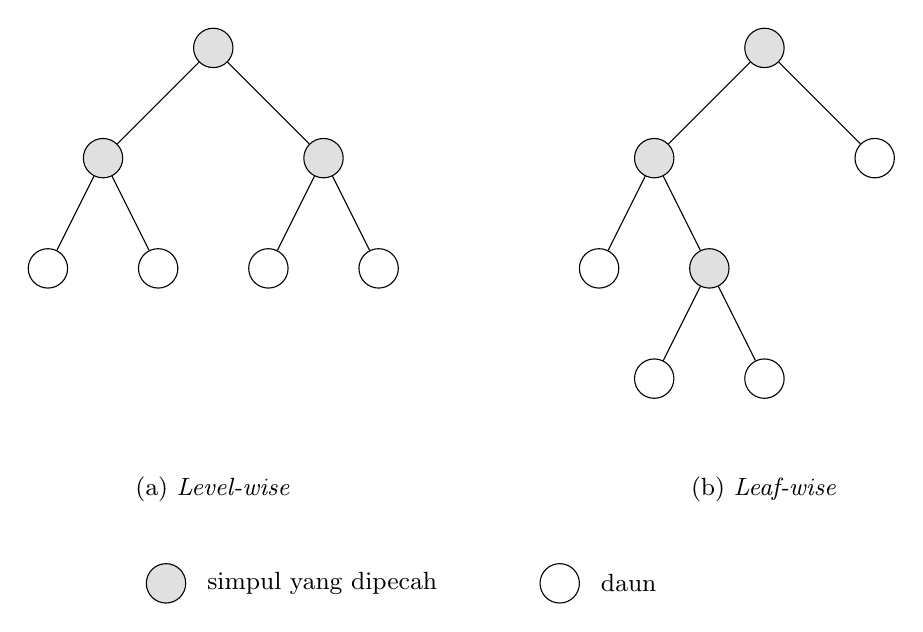
\begin{tikzpicture}[x=1mm,y=-1mm,
      simpul/.style={draw,circle,inner sep=0pt,minimum size=5mm},
      pecah/.style={draw,circle,fill=black!12,inner sep=0pt,minimum size=5mm}]
    % Panel kiri: level-wise
    \begin{scope}
      \node[pecah] (a) at (28,0) {};
      \node[pecah] (b) at (14,14) {};
      \node[pecah] (c) at (42,14) {};
      \node[simpul] (d) at (7,28) {};
      \node[simpul] (e) at (21,28) {};
      \node[simpul] (f) at (35,28) {};
      \node[simpul] (g) at (49,28) {};
      \draw (a) -- (b) (a) -- (c) (b) -- (d) (b) -- (e) (c) -- (f) (c) -- (g);
      \node[font=\small] at (28,56) {(a) \textit{Level-wise}};
    \end{scope}
    % Panel kanan: leaf-wise
    \begin{scope}[xshift=70mm]
      \node[pecah] (a2) at (28,0) {};
      \node[pecah] (b2) at (14,14) {};
      \node[simpul] (c2) at (42,14) {};
      \node[simpul] (d2) at (7,28) {};
      \node[pecah] (e2) at (21,28) {};
      \node[simpul] (f2) at (14,42) {};
      \node[simpul] (g2) at (28,42) {};
      \draw (a2) -- (b2) (a2) -- (c2) (b2) -- (d2) (b2) -- (e2)
            (e2) -- (f2) (e2) -- (g2);
      \node[font=\small] at (28,56) {(b) \textit{Leaf-wise}};
    \end{scope}
    % Legenda di bawah kedua panel.
    \node[pecah] (lg1) at (22,68) {};
    \node[anchor=west,font=\small] at (26,68) {simpul yang dipecah};
    \node[simpul] (lg2) at (72,68) {};
    \node[anchor=west,font=\small] at (76,68) {daun};
  \end{tikzpicture}
  \caption{Pertumbuhan Pohon \textit{Level-wise} dan \textit{Leaf-wise}}
  \label{fig:pohon-lgbm}
  \sumber{Digambar ulang, diadaptasi dari Ke dkk. \cite{ke2017}}
\end{figure}

LightGBM dipilih dengan tiga pertimbangan. Pertama, model berbasis pohon masih
unggul atas \textit{deep learning} pada data tabular berukuran kecil hingga
menengah \cite{grinsztajn2022}, dan data penelitian ini terdiri atas sekitar
3.000 observasi harian. Kedua, akurasinya setara dengan XGBoost
\cite{ke2017,chen2016}, sehingga pilihan di antara keduanya bukan inti
penelitian. Ketiga, sesuai arahan untuk menggunakan ML non-\textit{deep
learning}. Keunggulan kecepatan LightGBM tidak menjadi alasan pemilihan karena
dirancang untuk data besar. Model berbasis pohon juga cenderung meremehkan
volatilitas ekstrem \cite{dudek2024}, sehingga kekalahan model pada hari
lonjakan merupakan kemungkinan yang perlu diantisipasi.

% CEK: Grinsztajn dkk. (2022) dan Chen & Guestrin (2016) belum dicek.

\subsection{Fitur Berbasis Data Intraday}
Selain tiga komponen HAR, penelitian ini menggunakan fitur tambahan (fitur X)
yang seluruhnya diturunkan dari data OHLCV, karena prediktor internal pasar
terbukti paling penting dalam peramalan volatilitas kripto \cite{wang2023}.

\textit{Realized semivariance} negatif mengukur bagian variasi yang berasal
dari \textit{return} negatif \cite{barndorff2010}:
\begin{equation}
  RS_t^- = \sum_{i=1}^{288} r_{t,i}^2 \, \mathbf{1}(r_{t,i} < 0).
  \label{eq:semivarians}
\end{equation}
\begin{keterangan}
  \item[$RS_t^-$] \textit{realized semivariance} negatif pada hari $t$,
  \item[$\mathbf{1}(\cdot)$] fungsi indikator, bernilai 1 bila syarat di
    dalamnya terpenuhi dan 0 bila tidak.
\end{keterangan}
Patton dan Sheppard menunjukkan bahwa \textit{semivariance} negatif lebih
informatif untuk meramal volatilitas pada saham \cite{patton2015}. Karena
$RV_t = RS_t^- + RS_t^+$, fitur yang digunakan adalah proporsi $RS_t^-/RV_t$
agar tidak menimbulkan kolinearitas sempurna dengan komponen HAR.

Estimator \textit{range} Parkinson memanfaatkan harga tertinggi $P^{H}_t$ dan
terendah $P^{L}_t$ dalam satu hari \cite{parkinson1980}:
\begin{equation}
  \sigma^2_{P,t} = \frac{(\ln P^{H}_t - \ln P^{L}_t)^2}{4 \ln 2}.
  \label{eq:parkinson}
\end{equation}
\begin{keterangan}
  \item[$\sigma^2_{P,t}$] estimator varians \textit{range} Parkinson
    pada hari $t$,
  \item[$P^{H}_t$] harga tertinggi pada hari $t$,
  \item[$P^{L}_t$] harga terendah pada hari $t$.
\end{keterangan}
Estimator ini mengasumsikan perdagangan kontinu, asumsi yang lebih terpenuhi
pada Bitcoin yang diperdagangkan 24 jam sehari dibanding saham.

Ukuran \textit{illiquidity} Amihud mengukur dampak harga per satuan volume
transaksi \cite{amihud2002}. Mengikuti Do \cite{do2026}, ukuran ini dihitung
dalam versi \textit{realized} dari bar 5 menit:
\begin{equation}
  \text{Amihud}_t = 10^6 \cdot \frac{1}{N_t}\sum_{i}
  \frac{\left|r_{t,i}\right|}{QV_{t,i}},
  \label{eq:amihud}
\end{equation}
\begin{keterangan}
  \item[$\text{Amihud}_t$] ukuran \textit{illiquidity} pada hari $t$,
  \item[$r_{t,i}$] \textit{return} intraday pada bar ke-$i$,
  \item[$QV_{t,i}$] volume dalam dolar (USDT) pada bar ke-$i$,
  \item[$N_t$] jumlah bar bervolume positif pada hari $t$,
  \item[$10^6$] faktor penskalaan agar besarannya mudah dibaca.
\end{keterangan}
Amihud diperlakukan sebagai proksi dampak harga, bukan
biaya transaksi \cite{amihud2002,brauneis2021}. Fitur lainnya adalah
\textit{return} harian, logaritma volume dolar, dan perubahan logaritma volume.

\subsection{Fungsi Loss untuk Evaluasi Peramalan Volatilitas}
Karena volatilitas sebenarnya tidak teramati, evaluasi peramalan menggunakan
proksi RV. Patton menunjukkan bahwa hanya kelas fungsi \textit{loss} tertentu
yang menghasilkan peringkat model yang konsisten ketika proksi yang digunakan
berisik; dua anggota kelas tersebut adalah MSE dan QLIKE \cite{patton2011}.
Untuk ramalan $F_t$ dan proksi $RV_t$:
\begin{equation}
  L^{\text{QLIKE}}_t = \frac{RV_t}{F_t} - \ln\frac{RV_t}{F_t} - 1,
  \qquad
  L^{\text{MSE}}_t = (RV_t - F_t)^2.
  \label{eq:loss}
\end{equation}
\begin{keterangan}
  \item[$L^{\text{QLIKE}}_t$] nilai \textit{loss} QLIKE pada hari $t$,
  \item[$L^{\text{MSE}}_t$] nilai \textit{loss} MSE pada hari $t$,
  \item[$F_t$] ramalan RV untuk hari $t$,
  \item[$RV_t$] proksi volatilitas teramati pada Persamaan~\ref{eq:rv}.
\end{keterangan}
QLIKE homogen berderajat nol, artinya nilainya tidak berubah bila $RV_t$ dan
$F_t$ dikalikan konstanta yang sama, sehingga \textit{loss} tidak membesar
hanya karena volatilitas sedang tinggi. QLIKE juga menghukum ramalan yang
terlalu rendah lebih berat daripada ramalan yang terlalu tinggi dan memberikan
daya uji yang lebih tinggi \cite{patton2011}. Karena itu QLIKE digunakan sebagai
\textit{loss} utama dan MSE sebagai pelengkap. Ramalan optimal di bawah kedua
\textit{loss} tersebut adalah nilai harapan kondisional \cite{patton2011}.

Objek analisis penelitian ini adalah selisih \textit{loss} harian
\begin{equation}
  \Delta L_t = L_t(\text{ML}) - L_t(\text{HAR}),
  \label{eq:delta-loss}
\end{equation}
\begin{keterangan}
  \item[$\Delta L_t$] selisih \textit{loss} harian antara kedua model,
  \item[$L_t(\text{ML})$] \textit{loss} model \textit{machine learning}
    pada hari $t$,
  \item[$L_t(\text{HAR})$] \textit{loss} model HAR-RV pada hari $t$.
\end{keterangan}
Nilai $\Delta L_t$ yang negatif menunjukkan model ML lebih akurat pada hari
tersebut.
Karena kedua model dievaluasi pada hari dan proksi yang sama, $\Delta L_t$
tidak terpengaruh oleh perubahan skala volatilitas antarperiode.

\subsection{Uji Perbandingan Akurasi Peramalan}
Uji Diebold--Mariano (DM) menguji apakah dua model memiliki akurasi peramalan
yang sama, dengan hipotesis nol $E[\Delta L_t] = 0$ \cite{diebold1995}.
Statistik ujinya adalah
\begin{equation}
  DM = \frac{\overline{\Delta L}}{\sqrt{\widehat{V}_{\text{HAC}} / n}},
  \label{eq:dm}
\end{equation}
\begin{keterangan}
  \item[$DM$] statistik uji Diebold--Mariano,
  \item[$\overline{\Delta L}$] rata-rata selisih \textit{loss} selama
    periode uji,
  \item[$\widehat{V}_{\text{HAC}}$] estimator varians jangka panjang yang
    konsisten terhadap heteroskedastisitas dan autokorelasi,
  \item[$n$] jumlah observasi pada periode uji.
\end{keterangan}
Penelitian ini menggunakan estimator Newey--West \cite{newey1987} dengan \textit{bandwidth}
yang dipilih otomatis menurut Andrews \cite{andrews1991}.

Ketika sejumlah uji dijalankan sekaligus, peluang menemukan hasil signifikan
secara kebetulan meningkat. Prosedur Holm mengendalikan peluang tersebut dengan
mengurutkan \textit{p-value} dan membandingkannya dengan ambang yang makin
longgar secara bertahap \cite{holm1979}. Penelitian ini menetapkan uji
konfirmatori untuk setiap hipotesis sebelum melihat hasil
\textit{out-of-sample}. Hipotesis H2b terdiri atas dua uji sehingga
\textit{p-value}-nya dikoreksi dengan prosedur Holm, sedangkan uji lain
diperlakukan sebagai eksploratori dengan koreksi Holm.

% CEK: Diebold & Mariano (1995) dan Andrews (1991) belum dicek.

\subsection{Instabilitas Kinerja Peramalan dan Uji Perubahan Struktural}
Uji DM membandingkan akurasi rata-rata pada seluruh periode uji. Ketika
lingkungan berubah, kinerja relatif dua model dapat berbeda dari satu
subperiode ke subperiode lain, dan rata-rata keseluruhan dapat menyembunyikan
perubahan tersebut \cite{rossi2013}. Konsep ini perlu dibedakan dari
\textit{forecast breakdown}, yaitu kondisi ketika \textit{loss out-of-sample}
sebuah model secara signifikan lebih buruk daripada \textit{loss in-sample}-nya
\cite{giacomini2009}. Penelitian ini berfokus pada perubahan kinerja
\textbf{relatif} antarmodel, bukan pada kerusakan satu model.

\textit{Fluctuation test} dari Giacomini dan Rossi menghitung statistik DM
secara bergulir pada jendela berukuran $n_F = \mu n$ dan membandingkannya dengan
nilai kritis khusus yang memperhitungkan pengujian berulang
\cite{giacomini2010}. Uji ini menunjukkan kapan satu model lebih unggul, tetapi
hipotesis nolnya adalah kedua model sama akurat di setiap titik waktu, bukan
bahwa kinerja relatifnya stabil. Martins dan Perron menunjukkan bahwa daya uji
\textit{Fluctuation test} rendah dan tidak monoton setelah koreksi HAC, dan
mengusulkan penggunaan uji perubahan struktural pada rata-rata selisih
\textit{loss} \cite{martins2016}.

Uji perubahan struktural Bai--Perron menguji keberadaan perubahan rata-rata
$\Delta L_t$ pada titik waktu yang tidak diketahui \cite{bai1998}. Dengan
$\sup F_T(m)$ adalah statistik \textit{F} terbesar atas semua kemungkinan
penempatan $m$ titik patah, statistik UDmax didefinisikan sebagai
\begin{equation}
  \text{UDmax} = \max_{1 \le m \le M} \sup F_T(m),
  \label{eq:udmax}
\end{equation}
\begin{keterangan}
  \item[$\text{UDmax}$] statistik uji perubahan struktural maksimum,
  \item[$\sup F_T(m)$] statistik $F$ terbesar atas semua kemungkinan
    penempatan $m$ titik patah,
  \item[$M$] jumlah maksimum titik patah yang diuji.
\end{keterangan}
Statistik ini menguji hipotesis nol tanpa perubahan melawan alternatif adanya
satu hingga $M$ perubahan. Setiap segmen dibatasi minimal sebesar proporsi
\textit{trimming} $\varepsilon$ dari sampel. Bai dan Perron menganjurkan UDmax
dijalankan lebih dahulu; bila menolak, jumlah titik patah ditentukan dengan uji
berurutan $\sup F(\ell+1 \mid \ell)$ \cite{bai2003}. Penelitian ini menggunakan
UDmax sebagai uji konfirmatori kestabilan dan \textit{Fluctuation test} sebagai
visualisasi eksploratori.

% CEK: Giacomini & Rossi (2010) baru metadata. Deskripsi mekanisme Fluctuation
% test diambil dari Martins & Perron (2016) dan Rossi (2013) yang sudah full
% text.

\subsection{Evaluasi Out-of-Sample dan Strategi Pembaruan Model}
Evaluasi model peramalan deret waktu harus menghormati urutan waktu. Tashman
menekankan pentingnya evaluasi \textit{out-of-sample} dengan banyak titik asal
peramalan, dan membedakan \textit{updating}, yaitu memasukkan data baru tanpa
mengestimasi ulang parameter, dari \textit{recalibration}, yaitu mengestimasi
ulang parameter dengan data terbaru \cite{tashman2000}. Untuk data yang tidak
stasioner, Cerqueira, Torgo, dan Mozetič merekomendasikan skema
\textit{out-of-sample} berurutan dan validasi \textit{forward-chaining}, bukan
validasi silang acak, karena pengacakan memungkinkan informasi masa depan bocor
ke data latih \cite{cerqueira2020}.

Dalam literatur \textit{concept drift}, cara model beradaptasi terhadap data
yang berubah dikelompokkan antara lain berdasarkan pengelolaan \textit{window}
data latih \cite{gama2014}. \textit{Window} yang tumbuh (\textit{landmark} atau
\textit{expanding}) menyimpan seluruh histori, sedangkan \textit{window} geser
berukuran tetap (\textit{rolling}) hanya memakai data terbaru. Model yang tidak
pernah dilatih ulang berfungsi sebagai pembanding untuk mengukur manfaat
adaptasi \cite{zliobaite2015}. Tabel~\ref{tab:strategi} dan
Gambar~\ref{fig:strategi} merangkum ketiga strategi yang digunakan.

\begin{table}[htbp]
  \caption{Strategi Pembaruan Model dan Padanannya dalam Literatur}
  \label{tab:strategi}
  \centering
  \begingroup
  \setstretch{1}\small
  \begin{tabular}{|c|l|p{0.3\textwidth}|p{0.32\textwidth}|}
    \hline
    \textbf{Kode} & \textbf{Strategi} & \textbf{Data latih} &
    \textbf{Padanan dalam literatur} \\
    \hline
    S0 & Static & Dilatih sekali pada window awal, tidak dilatih ulang &
    \textit{Updating} tanpa rekalibrasi \cite{tashman2000}; pembanding manfaat
    adaptasi \cite{zliobaite2015} \\
    \hline
    S1 & Expanding & Dilatih ulang bulanan dengan seluruh data yang tersedia &
    \textit{Landmark} atau \textit{growing window}
    \cite{gama2014,cerqueira2020} \\
    \hline
    S2 & Rolling & Dilatih ulang bulanan dengan $W$ hari terakhir,
    $W \in \{365, 730\}$; uji konfirmatori memakai $W = 365$ (S2-365) &
    \textit{Fixed-size sliding window} \cite{gama2014} \\
    \hline
  \end{tabular}
  \endgroup
\end{table}

\begin{figure}[htbp]
  \centering
  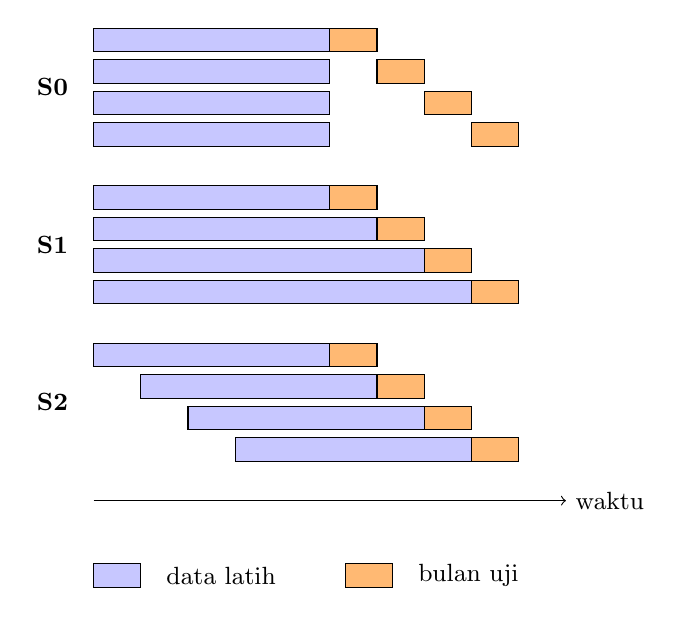
\begin{tikzpicture}[x=1mm,y=-1mm]
    % Sumbu y dibalik (y=-1mm), sehingga posisi baris dihitung langsung di
    % sini; jangan memakai yshift pada scope karena arahnya tidak ikut dibalik.
    \tikzset{
      latih/.style={draw,fill=blue!22},
      uji/.style={draw,fill=orange!55}}
    % Tiga strategi, masing-masing empat iterasi bulanan.
    % S0 baris 0--12, S1 baris 20--32, S2 baris 40--52.
    \foreach \i in {0,...,3} {
      \pgfmathsetmacro\y{\i*4}
      \pgfmathsetmacro\ujix{30+\i*6}
      % S0: data latih tetap pada window awal
      \filldraw[latih] (0,\y) rectangle (30,\y+3);
      \filldraw[uji] (\ujix,\y) rectangle (\ujix+6,\y+3);
      % S1: data latih memanjang dari titik awal
      \filldraw[latih] (0,\y+20) rectangle (\ujix,\y+23);
      \filldraw[uji] (\ujix,\y+20) rectangle (\ujix+6,\y+23);
      % S2: data latih berukuran tetap yang bergeser
      \filldraw[latih] (\i*6,\y+40) rectangle (\i*6+30,\y+43);
      \filldraw[uji] (\ujix,\y+40) rectangle (\ujix+6,\y+43);
    }
    \node[anchor=east,font=\small\bfseries] at (-2,7.5) {S0};
    \node[anchor=east,font=\small\bfseries] at (-2,27.5) {S1};
    \node[anchor=east,font=\small\bfseries] at (-2,47.5) {S2};
    % Sumbu waktu dan legenda
    \draw[->] (0,60) -- (60,60) node[right,font=\small] {waktu};
    \filldraw[latih] (0,68) rectangle (6,71);
    \node[anchor=west,font=\small] at (8,69.5) {data latih};
    \filldraw[uji] (32,68) rectangle (38,71);
    \node[anchor=west,font=\small] at (40,69.5) {bulan uji};
  \end{tikzpicture}
  \caption{Skema Strategi Pembaruan Model Static, Expanding, dan Rolling}
  \label{fig:strategi}
\end{figure}

Pilihan strategi melibatkan \textit{trade-off} bias dan varians. Pesaran dan
Timmermann, sebagaimana dirangkum Rossi, menunjukkan bahwa data sebelum
perubahan struktural menambah bias tetapi mengurangi varians estimasi;
\textit{rolling window} cenderung lebih baik ketika perubahan besar dan
berulang, sedangkan skema rekursif (\textit{expanding}) lebih baik ketika
perubahan kecil \cite{rossi2013}. Untuk model autoregresif seperti HAR, data
sebelum perubahan bahkan dapat mengurangi bias dan varians sekaligus
\cite{rossi2013}. Pilihan \textit{window} pada perbandingan ML dengan HAR juga
harus setara, karena HAR yang diberi skema \textit{fitting} yang kurang tepat
dapat membuat ML tampak unggul secara semu \cite{chassot2026}. Kerangka uji
perbandingan peramalan Giacomini--White dirumuskan untuk skema \textit{rolling}
atau \textit{fixed} \cite{rossi2013}, dan skema \textit{rolling} menyamakan
panjang data latih antarperiode \cite{tashman2000}; karena itu uji formal
kestabilan dijalankan pada skema \textit{rolling}.

\subsection{Pergeseran Distribusi Data}
Pergeseran data (\textit{dataset shift}) terjadi ketika distribusi bersama
masukan dan target pada data uji berbeda dari data latih
\cite{morenotorres2012}. Literatur menggunakan istilah yang berbeda untuk jenis
perubahan yang sama, seperti dirangkum pada Tabel~\ref{tab:istilah}.

\begin{table}[htbp]
  \caption{Perbandingan Istilah Pergeseran Data menurut Gama dkk. dan
    Moreno-Torres dkk.}
  \label{tab:istilah}
  \centering
  \begingroup
  \setstretch{1}\small
  \begin{tabular}{|l|p{0.33\textwidth}|p{0.33\textwidth}|}
    \hline
    \textbf{Perubahan} & \textbf{Gama dkk. \cite{gama2014}} &
    \textbf{Moreno-Torres dkk. \cite{morenotorres2012}} \\
    \hline
    $P(x)$ berubah & \textit{Virtual drift} (tanpa syarat mengenai
    $P(y \mid x)$) & \textit{Covariate shift} (dengan syarat $P(y \mid x)$
    tetap) \\
    \hline
    $P(y \mid x)$ berubah & \textit{Real concept drift} ($P(x)$ boleh berubah) &
    \textit{Concept shift} (dengan syarat $P(x)$ tetap) \\
    \hline
  \end{tabular}
  \endgroup
\end{table}

Peramalan RV termasuk masalah $X \rightarrow Y$, karena fitur hari $t$
mendahului target hari $t+1$, sehingga kerangka Moreno-Torres dkk. yang relevan
\cite{morenotorres2012}. Penelitian ini hanya mengukur perubahan distribusi
fitur $P(x)$ dan tidak menguji apakah $P(y \mid x)$ tetap. Oleh karena itu
istilah yang dipakai adalah \textbf{pergeseran distribusi fitur}, bukan
\textit{covariate shift} atau \textit{concept drift} dalam arti formal.

Pergeseran distribusi satu fitur antara data latih dan bulan uji diukur dengan
statistik Kolmogorov--Smirnov dua sampel,
\begin{equation}
  D^{\text{KS}} = \sup_x
  \left| \hat{F}_{\text{latih}}(x) - \hat{F}_{\text{uji}}(x) \right|,
  \label{eq:ks}
\end{equation}
\begin{keterangan}
  \item[$D^{\text{KS}}$] statistik Kolmogorov--Smirnov dua sampel,
  \item[$\hat{F}_{\text{latih}}(x)$] fungsi distribusi kumulatif empiris
    data latih,
  \item[$\hat{F}_{\text{uji}}(x)$] fungsi distribusi kumulatif empiris
    bulan uji,
  \item[$\sup_x$] nilai terbesar atas seluruh $x$.
\end{keterangan}
Nilai $D^{\text{KS}}$ adalah jarak terbesar antara kedua fungsi distribusi
kumulatif empiris. Uji KS per
fitur merupakan salah satu pendekatan untuk mendeteksi pergeseran data
\cite{rabanser2019}. Nilai $D^{\text{KS}}$ dirata-ratakan antarfitur untuk
memperoleh satu ukuran pergeseran per bulan.

% CEK: Rabanser dkk. (2019) belum dicek.

\subsection{Proksi Likuiditas}
\label{subsec:likuiditas}
Likuiditas pasar kripto dapat diukur dengan berbagai proksi berbasis data harga
dan volume. Brauneis dkk. menunjukkan bahwa proksi yang paling baik menangkap
variasi likuiditas kripto antarwaktu berbeda dengan proksi yang paling baik
menangkap levelnya: estimator \textit{spread} Abdi--Ranaldo unggul untuk
variasi waktu, sedangkan ukuran Amihud unggul untuk level \cite{brauneis2021}.
Karena itu, penelitian ini memakai Amihud sebagai fitur model LGBM-X dan
estimator
Abdi--Ranaldo, yang dihitung dari harga OHLC harian, sebagai variabel likuiditas
dalam analisis asosiasi kinerja relatif dengan kondisi pasar, dengan estimator
Corwin--Schultz sebagai uji sensitivitas. Amihud tidak disertakan pada HAR-X
karena berkolinearitas tinggi dengan komponen HAR berdasarkan pemeriksaan pada
\textit{window} awal; rinciannya diuraikan pada Bab III. Proksi likuiditas harian juga
dipakai Zhang dkk. untuk mengkaji hubungan antara \textit{return} dan
likuiditas aset kripto \cite{zhang2024}.

% CEK: Paper asli estimator Abdi--Ranaldo (2017) dan Corwin--Schultz (2012)
% belum ada di daftar referensi. Tambahkan ke references.bib setelah
% diverifikasi; sementara klaim disandarkan pada Brauneis dkk. (2021).

\section{Kerangka Pemikiran}
Kerangka pemikiran penelitian ini berangkat dari dua fakta. Pertama,
karakteristik pasar Bitcoin berubah lintas era \cite{do2026,mokni2024}. Kedua,
perbandingan model ML dengan HAR-RV umumnya dilaporkan sebagai satu hasil
agregat \cite{dudek2024,huang2024}, padahal kinerja relatif dapat berubah
sepanjang waktu \cite{rossi2013,gama2014}. Dari kedua fakta tersebut,
penelitian ini menanyakan apakah kinerja relatif LightGBM terhadap HAR-RV
stabil, faktor pasar apa yang berasosiasi dengan perubahannya, dan bagaimana
strategi pembaruan model memengaruhinya.

Untuk menjawabnya, perbedaan kinerja diurai melalui desain $2 \times 2$ pada
Tabel~\ref{tab:desain}. Perbandingan LGBM-HAR dengan HAR mengukur kontribusi
non-linearitas, perbandingan HAR-X dengan HAR mengukur kontribusi informasi
tambahan, dan perbandingan LGBM-X dengan HAR mengukur kontribusi total. Model
\textit{naive persistence} ($\widehat{RV}_{t+1} = RV_t$) disertakan sebagai
pemeriksaan kewajaran \cite{gama2014}.

\begin{table}[htbp]
  \caption{Desain Perbandingan Model $2 \times 2$}
  \label{tab:desain}
  \centering
  \begingroup
  \setstretch{1}
  \begin{tabular}{|l|c|c|}
    \hline
    & \textbf{Masukan HAR} & \textbf{Masukan HAR + fitur X} \\
    \hline
    \textbf{Linear} & HAR-RV (pembanding) & HAR-X \\
    \hline
    \textbf{Non-linear} & LGBM-HAR & LGBM-X \\
    \hline
  \end{tabular}
  \endgroup
\end{table}

Pada HAR-X, fitur X tidak mencakup ukuran Amihud (lihat
Subbab~\ref{subsec:likuiditas}).

Alur kerangka pemikiran ditunjukkan pada Gambar~\ref{fig:kerangka}.

\begin{figure}[htbp]
  \centering
  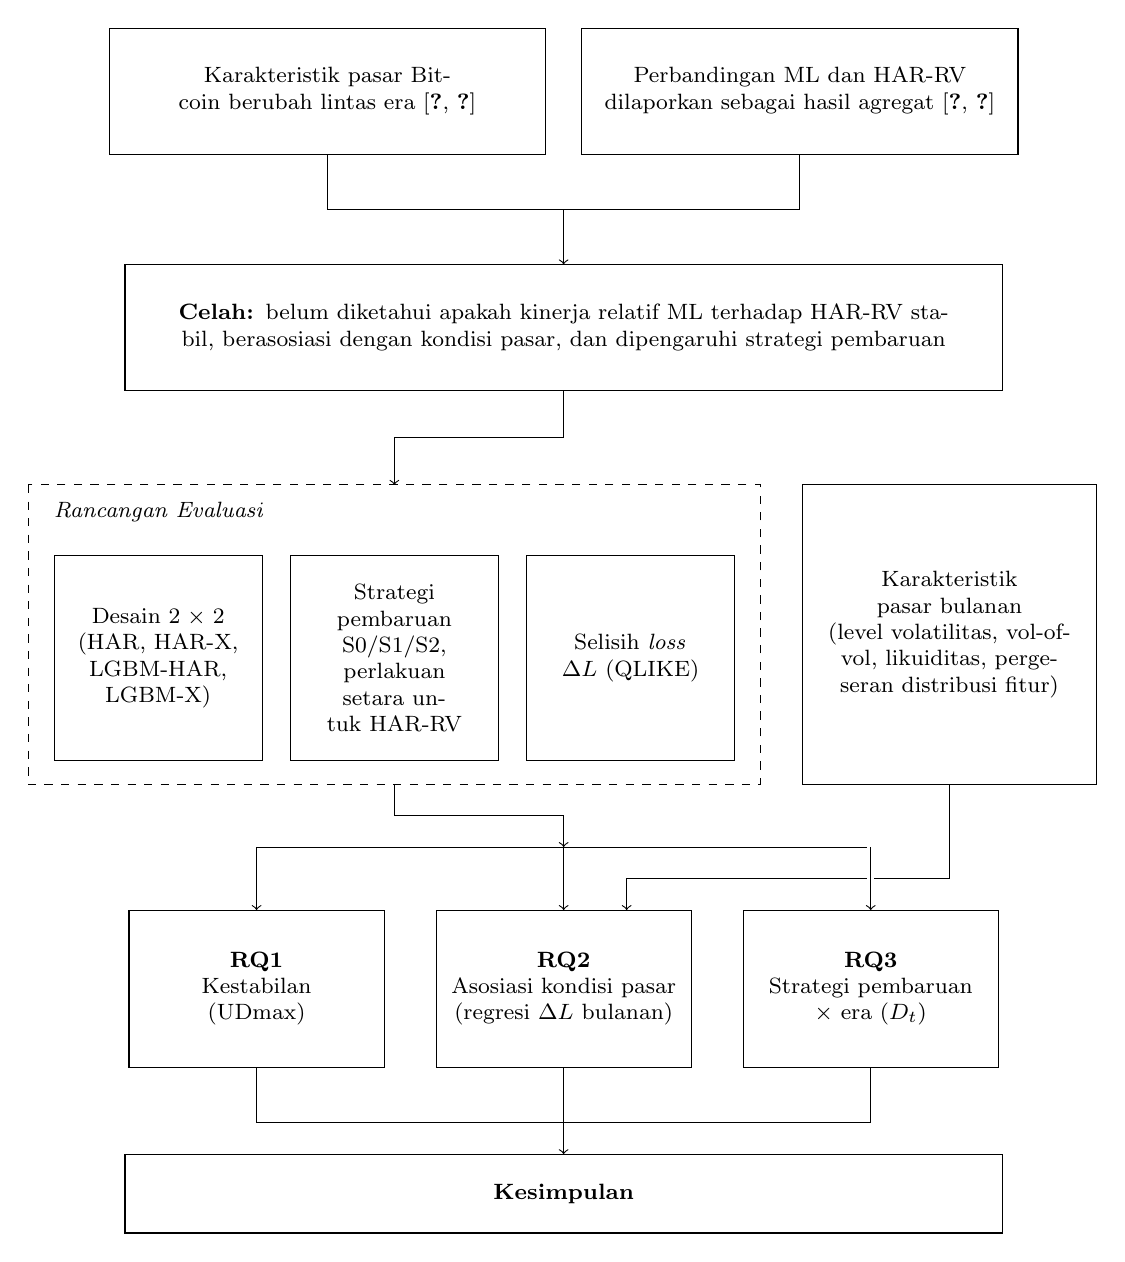
\begin{tikzpicture}[x=1mm,y=-1mm,
      kotak/.style={draw,align=center,inner sep=2pt,font=\footnotesize},
      fakta/.style={kotak,text width=54mm,minimum height=16mm},
      lebar/.style={kotak,text width=110mm},
      komponen/.style={kotak,text width=25mm,minimum height=26mm},
      pasar/.style={kotak,text width=36mm,minimum height=38mm},
      rq/.style={kotak,text width=31mm,minimum height=20mm}]

    % --- Baris 1: dua fakta pembuka yang berdiri sejajar ---------------------
    \node[fakta] (faktaa) at (-30,0)
      {Karakteristik pasar Bitcoin berubah lintas era
       \cite{do2026,mokni2024}};
    \node[fakta] (faktab) at (30,0)
      {Perbandingan ML dan HAR-RV dilaporkan sebagai hasil agregat
       \cite{dudek2024,huang2024}};

    % --- Baris 2: celah tempat kedua fakta bertemu ---------------------------
    \node[lebar,minimum height=16mm] (celah) at (0,30)
      {\textbf{Celah:} belum diketahui apakah kinerja relatif ML terhadap
       HAR-RV stabil, berasosiasi dengan kondisi pasar, dan dipengaruhi
       strategi pembaruan};

    % --- Baris 3: wadah rancangan evaluasi dan masukan karakteristik pasar ---
    \draw[dashed] (-68,50) rectangle (25,88);
    \node[anchor=north west,font=\footnotesize\itshape] at (-66,51)
      {Rancangan Evaluasi};
    \node[komponen] at (-51.5,72)
      {Desain $2 \times 2$\\(HAR, HAR-X,\\LGBM-HAR, LGBM-X)};
    \node[komponen] at (-21.5,72)
      {Strategi pembaruan\\S0/S1/S2, perlakuan\\setara untuk HAR-RV};
    \node[komponen] at (8.5,72)
      {Selisih \textit{loss}\\$\Delta L$ (QLIKE)};
    \node[pasar] (pasar) at (49,69)
      {Karakteristik pasar bulanan\\(level volatilitas, vol-of-vol,
       likuiditas, pergeseran distribusi fitur)};

    % --- Baris 4: tiga rumusan masalah --------------------------------------
    \node[rq] (rq1) at (-39,114) {\textbf{RQ1}\\Kestabilan\\(UDmax)};
    \node[rq] (rq2) at (0,114)
      {\textbf{RQ2}\\Asosiasi kondisi pasar\\(regresi $\Delta L$ bulanan)};
    \node[rq] (rq3) at (39,114)
      {\textbf{RQ3}\\Strategi pembaruan\\$\times$ era ($D_t$)};

    % --- Baris 5: kesimpulan, sengaja generik karena bab ini pra-hasil ------
    \node[lebar,minimum height=10mm] (simpulan) at (0,140) {\textbf{Kesimpulan}};

    % --- Panah --------------------------------------------------------------
    % Kedua fakta bertemu di satu titik sebelum masuk ke kotak celah.
    \draw (-30,8) -- (-30,15);
    \draw (30,8) -- (30,15);
    \draw (-30,15) -- (30,15);
    \draw[->] (0,15) -- (0,22);
    % Celah mengarah ke wadah rancangan evaluasi.
    \draw (0,38) -- (0,44) -- (-21.5,44);
    \draw[->] (-21.5,44) -- (-21.5,50);
    % Satu panah dari wadah ke baris RQ, lalu dibagikan ke ketiga kotak.
    \draw (-21.5,88) -- (-21.5,92) -- (0,92);
    \draw[->] (0,92) -- (0,96);
    \draw (-39,96) -- (39,96);
    \draw[->] (-39,96) -- (-39,104);
    \draw[->] (0,96) -- (0,104);
    % Karakteristik pasar hanya memberi masukan ke RQ2.
    \draw[->] (49,88) -- (49,100) -- (8,100) -- (8,104);
    % Digambar terakhir dengan halo putih agar tampak melompati garis di atas.
    \draw[white,line width=2.4pt] (39,96) -- (39,104);
    \draw[->] (39,96) -- (39,104);
    % Ketiga RQ bermuara pada satu kesimpulan.
    \draw (-39,124) -- (-39,131);
    \draw (0,124) -- (0,131);
    \draw (39,124) -- (39,131);
    \draw (-39,131) -- (39,131);
    \draw[->] (0,131) -- (0,135);
  \end{tikzpicture}
  \caption{Kerangka Pemikiran Penelitian}
  \label{fig:kerangka}
\end{figure}

\section{Hipotesis Penelitian}
Berdasarkan landasan teori di atas, hipotesis penelitian dirumuskan sebagai
berikut.

\textbf{H1.} Rata-rata selisih \textit{loss}
$\Delta L(\text{LGBM-X} - \text{HAR})$ tidak konstan sepanjang periode
pengujian. Hipotesis ini diturunkan dari perubahan karakteristik pasar Bitcoin
lintas era \cite{do2026,mokni2024} dan dari literatur instabilitas peramalan
\cite{rossi2013,martins2016}.

\textbf{H2a.} Selisih \textit{loss} bulanan berasosiasi dengan sedikitnya satu
karakteristik pasar, yaitu level volatilitas, volatilitas dari volatilitas,
likuiditas, atau pergeseran distribusi fitur. Pendekatan meregresikan ukuran
kinerja peramalan pada indikator yang teramati mengikuti semangat Giacomini dan
Rossi \cite{giacomini2009}.

\textbf{H2b.} Kontribusi fitur X terhadap kinerja relatif berbeda antara era
\textit{transition} dan \textit{institutional}. Do menunjukkan bahwa hubungan
volatilitas--likuiditas berubah antarera \cite{do2026}, tetapi Do menguji arah
volatilitas terhadap \textit{illiquidity}, sedangkan penelitian ini memakai
likuiditas dan volume untuk meramal RV; H2b merupakan perluasan dari temuan
tersebut. Mokni dkk. menunjukkan hubungan likuiditas dapat berbalik tanda
\cite{mokni2024}, dan kepentingan fitur tidak konsisten antarstudi
\cite{wang2023,feng2024ml}. Karena itu H2b dirumuskan dua arah.

\textbf{H3.} Pada era \textit{institutional}, kinerja relatif LGBM-X terhadap
HAR-RV lebih baik pada strategi \textit{rolling} 365 hari (S2-365)
dibandingkan \textit{expanding} (S1). Dengan
$D_t = \Delta L_t(\text{S2-365}) - \Delta L_t(\text{S1})$, dan $\Delta L_t$
adalah selisih \textit{loss} LGBM-X terhadap HAR-RV pada
Persamaan~\ref{eq:delta-loss}, H3 didukung bila rata-rata $D_t$ negatif dan
signifikan. Hipotesis ini
didasarkan pada \textit{trade-off} bias--varians \cite{rossi2013} dan perubahan
persistensi RV antarera \cite{do2026}: hubungan yang dipelajari dari era awal
dapat usang, dan LGBM-X yang lebih fleksibel diduga lebih terdampak data usang
daripada HAR.

\textbf{Hipotesis tandingan.} Hasil yang berlawanan dengan H3 tetap bermakna.
Untuk model autoregresif, data sebelum perubahan struktural dapat mengurangi
bias dan varians sekaligus, sehingga skema \textit{expanding} dapat lebih baik
daripada \textit{rolling} \cite{rossi2013}. Selain itu, bila \textit{regime}
volatilitas berulang, data lama tetap relevan \cite{gama2014,suarez2023}.

Ringkasan rumusan masalah, hipotesis, dan uji konfirmatorinya disajikan pada
Tabel~\ref{tab:ringkasan}. Uji konfirmatori ditetapkan sebelum hasil
\textit{out-of-sample} dilihat.

\begin{table}[htbp]
  \caption{Ringkasan Rumusan Masalah, Hipotesis, dan Uji Konfirmatori}
  \label{tab:ringkasan}
  \centering
  \begingroup
  \setstretch{1}\small
  \begin{tabular}{|p{0.22\textwidth}|c|p{0.47\textwidth}|}
    \hline
    \textbf{Rumusan masalah} & \textbf{Hipotesis} &
    \textbf{Uji konfirmatori} \\
    \hline
    RQ1 Kestabilan kinerja relatif & H1 &
    UDmax pada rata-rata $\Delta L(\text{LGBM-X} - \text{HAR})$, skema rolling
    365 hari, QLIKE, HAC, $\varepsilon = 0{,}15$, maksimum 5 perubahan; bila
    tidak menolak, uji DM pada seluruh sampel \\
    \hline
    RQ2 Asosiasi dengan kondisi pasar & H2a, H2b &
    H2a: uji-F bersama (HAC) pada regresi $\Delta L$ bulanan terhadap
    4 karakteristik pasar. H2b: dua uji-t HAC beda rata-rata antara era
    \textit{transition} dan \textit{institutional}, untuk
    $\Delta L(\text{HAR-X} - \text{HAR})$ dan
    $\Delta L(\text{LGBM-X} - \text{LGBM-HAR})$, dengan koreksi Holm \\
    \hline
    RQ3 Strategi pembaruan $\times$ era & H3 &
    Uji-t HAC dua sisi pada rata-rata
    $D_t = \Delta L_t(\text{S2-365}) - \Delta L_t(\text{S1})$ pasangan LGBM-X
    dan HAR-RV di era \textit{institutional} \\
    \hline
  \end{tabular}
  \endgroup
\end{table}

\chapter{Metodologi}

Bab ini menguraikan rancangan penelitian yang digunakan untuk menjawab ketiga
rumusan masalah pada Subbab 1.2, meliputi jenis dan alur penelitian, data,
rancangan model dan skema pembaruan, contoh perhitungan, serta rancangan
evaluasi dan pengujian hipotesis.

\section{Metode Penelitian}
Penelitian ini merupakan penelitian kuantitatif eksperimental dengan data
sekunder deret waktu. Objek yang dievaluasi adalah kinerja relatif model
LightGBM terhadap model HAR-RV dalam meramalkan \textit{realized variance}
harian BTC/USDT spot satu hari ke depan. Penelitian bersifat implementatif:
seluruh tahapan, mulai dari pengolahan data, pelatihan model, hingga pengujian
statistik, diimplementasikan sebagai satu \textit{pipeline} perangkat lunak
yang dapat dijalankan ulang.

Seluruh keputusan desain, termasuk pasangan model, skema, fungsi \textit{loss},
dan uji konfirmatori untuk setiap hipotesis (Tabel~\ref{tab:ringkasan}),
ditetapkan dalam satu berkas konfigurasi sebelum hasil \textit{out-of-sample}
pasangan konfirmatori dilihat. Nilai \textit{hash} berkas konfigurasi dicatat
pada setiap keluaran sehingga perubahan desain setelah hasil diketahui dapat
terdeteksi. Prinsip ini mencegah pemilihan uji atau hipotesis berdasarkan
hasil.

\subsection{Alur Penelitian}
Alur penelitian ditunjukkan pada Gambar~\ref{fig:alur} dan terdiri atas
tahapan berikut: (1) pengunduhan data dan verifikasi \textit{checksum};
(2) audit dan pembentukan tabel harian; (3) pembentukan target dan fitur;
(4) pemeriksaan kolinearitas dan \textit{tuning hyperparameter} pada
\textit{window} awal; (5) peramalan \textit{walk-forward} untuk setiap skema
pembaruan dan model; (6) perhitungan \textit{loss} harian dan selisih
\textit{loss}; (7) pengujian hipotesis konfirmatori dan analisis eksploratori
untuk RQ1--RQ3.

\begin{figure}[htbp]
  \centering
  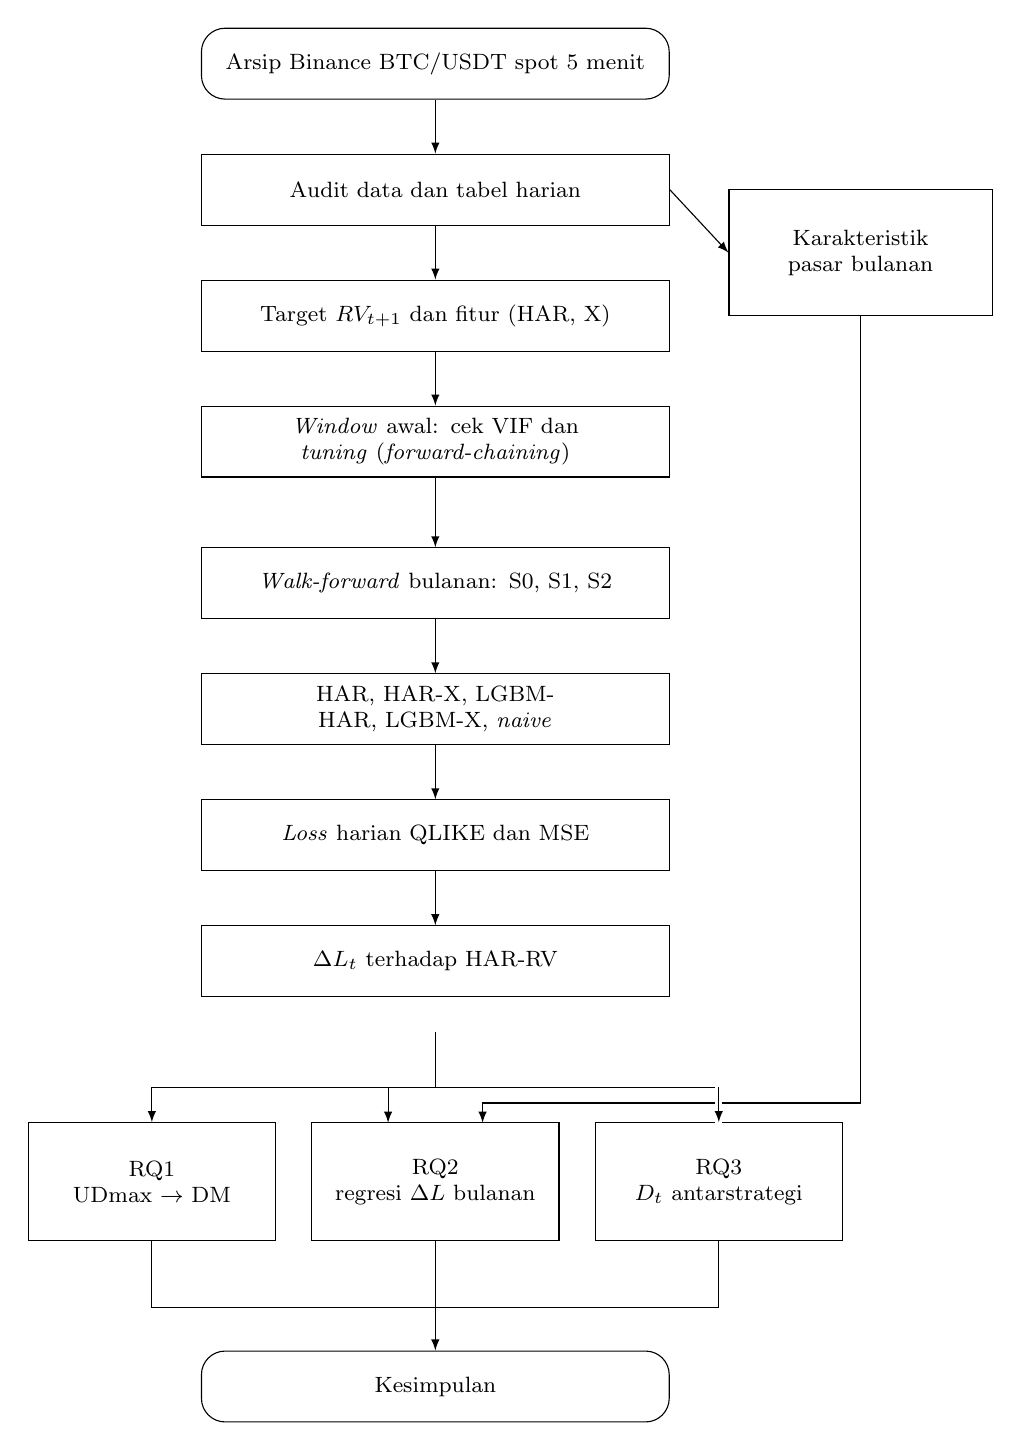
\begin{tikzpicture}[x=1mm,y=-1mm,
      kotak/.style={draw,align=center,inner sep=2pt,font=\footnotesize,
        text width=58mm,minimum height=9mm},
      ujung/.style={kotak,rounded corners=3mm},
      sisi/.style={draw,align=center,inner sep=2pt,font=\footnotesize,
        text width=32mm,minimum height=16mm},
      rq/.style={draw,align=center,inner sep=2pt,font=\footnotesize,
        text width=30mm,minimum height=15mm},
      pn/.style={->,>=latex}]

    % Kolom utama
    \node[ujung] (n1) at (0,0)
      {Arsip Binance BTC/USDT spot 5 menit};
    \node[kotak] (n2) at (0,16) {Audit data dan tabel harian};
    \node[kotak] (n3) at (0,32) {Target $RV_{t+1}$ dan fitur (HAR, X)};
    \node[kotak] (n4) at (0,48)
      {\textit{Window} awal: cek VIF dan \textit{tuning}
       (\textit{forward-chaining})};
    \node[kotak] (n5) at (0,66)
      {\textit{Walk-forward} bulanan: S0, S1, S2};
    \node[kotak] (n6) at (0,82)
      {HAR, HAR-X, LGBM-HAR, LGBM-X, \textit{naive}};
    \node[kotak] (n7) at (0,98) {\textit{Loss} harian QLIKE dan MSE};
    \node[kotak] (n8) at (0,114) {$\Delta L_t$ terhadap HAR-RV};

    % Masukan samping khusus RQ2
    \node[sisi] (pasar) at (54,24) {Karakteristik\\pasar bulanan};

    % Tiga rumusan masalah
    \node[rq] (rq1) at (-36,142) {RQ1\\UDmax $\rightarrow$ DM};
    \node[rq] (rq2) at (0,142) {RQ2\\regresi $\Delta L$ bulanan};
    \node[rq] (rq3) at (36,142) {RQ3\\$D_t$ antarstrategi};

    \node[ujung] (simp) at (0,168) {Kesimpulan};

    % Panah kolom utama
    \foreach \a/\b in {n1/n2, n2/n3, n3/n4, n4/n5, n5/n6, n6/n7, n7/n8}
      {\draw[pn] (\a) -- (\b);}

    % Audit data memasok karakteristik pasar bulanan
    \draw[pn] (n2.east) -- (pasar.west);

    % Satu panah dari delta L, lalu dibagikan ke ketiga RQ
    \draw (0,123) -- (0,130);
    \draw (-36,130) -- (36,130);
    \draw[pn] (-36,130) -- (rq1.north);
    \draw[pn] (-6,130) -- (-6,134.5);
    % Karakteristik pasar hanya memberi masukan ke RQ2; digambar lebih dulu
    % agar garis RQ3 di bawah tampak melompatinya.
    \draw[pn] (pasar.south) -- (54,132) -- (6,132) -- (6,134.5);
    \draw[white,line width=2.4pt] (36,130) -- (36,134.5);
    \draw[pn] (36,130) -- (rq3.north);

    % Ketiga RQ bermuara pada kesimpulan
    \draw (-36,149.5) -- (-36,158);
    \draw (0,149.5) -- (0,158);
    \draw (36,149.5) -- (36,158);
    \draw (-36,158) -- (36,158);
    \draw[pn] (0,158) -- (simp.north);
  \end{tikzpicture}
  \caption{Alur Penelitian}
  \label{fig:alur}
\end{figure}

\subsection{Tahap Uji Kelayakan}
Sebelum desain dikunci, dilakukan tahap uji kelayakan dengan pasangan
eksploratori LGBM-HAR dan HAR-RV. Tahap ini memeriksa kelengkapan data,
kebenaran \textit{pipeline}, kolinearitas fitur, prosedur \textit{tuning}, dan
daya uji. Pasangan konfirmatori LGBM-X terhadap HAR-RV tidak dievaluasi secara
\textit{out-of-sample} pada tahap tersebut, dan hasil uji kelayakan tidak
digunakan untuk mengubah rumusan masalah, hipotesis, maupun uji konfirmatori.

% CEK: tahap ini wajib diungkap terbuka (lihat hasil_eksperimen par. 5).
% Jangan menambahkan angka hasil pilot.

\subsection{Peralatan Penelitian}
Implementasi menggunakan bahasa Python 3.12 dengan pustaka \texttt{pandas},
\texttt{numpy}, \texttt{lightgbm} (versi 4 ke atas), \texttt{scikit-learn},
\texttt{statsmodels}, \texttt{scipy}, dan \texttt{matplotlib}. Estimator
kovarians HAC diimplementasikan sendiri mengikuti kernel Bartlett dengan
\textit{bandwidth} otomatis Andrews \cite{andrews1991} dan diverifikasi
menghasilkan nilai yang identik dengan fungsi \texttt{kernHAC} paket R
\texttt{sandwich}. Seluruh pelatihan memakai \textit{seed} tetap (42) dan mode
deterministik LightGBM.

% CEK: spesifikasi perangkat keras (laptop/OS) bila diminta pedoman; isi dari
% Ferdi.

\section{Desain Sistem}

\subsection{Data}
Data yang digunakan adalah \textit{klines} (OHLCV) BTC/USDT pasar spot dengan
resolusi 5 menit dari arsip publik Binance (\texttt{data.binance.vision}),
diunduh per bulan dan diverifikasi dengan \textit{checksum} SHA-256 resmi.
Periode data adalah 17 Agustus 2017, yaitu awal ketersediaan arsip, hingga
30 September 2026. Kolom yang digunakan adalah harga pembukaan, tertinggi,
terendah, penutupan, serta \textit{quote asset volume} (volume dalam USDT)
sebagai volume dolar. Ringkasan data ditunjukkan pada Tabel~\ref{tab:data} dan
pergerakannya pada Gambar~\ref{fig:data}.

\begin{table}[htbp]
  \caption{Ringkasan Data Penelitian}
  \label{tab:data}
  \centering
  \begingroup
  \setstretch{1}
  \begin{tabular}{|l|p{0.52\textwidth}|}
    \hline
    \textbf{Komponen} & \textbf{Keterangan} \\
    \hline
    Sumber & Binance Public Data, folder \textit{spot}, simbol berkas
      BTCUSDT \\
    \hline
    Resolusi & 5 menit (288 bar per hari UTC) \\
    \hline
    Periode & 17 Agustus 2017 -- 30 September 2026 \\
    \hline
    Jumlah bar & 957.865 \\
    \hline
    Jumlah hari & 3.332 \\
    \hline
    Hari dengan bar $<$ 95\% & 27 (dibuang, Subbab~\ref{subsec:audit}) \\
    \hline
    Hari dengan $RV = 0$ & 0 \\
    \hline
  \end{tabular}
  \endgroup
\end{table}

Pemilihan pasar spot didasarkan pada tiga alasan: histori spot tersedia sejak
2017 sementara kontrak \textit{perpetual} baru sejak sekitar September 2019,
padahal RQ3 membutuhkan data era awal; harga \textit{perpetual} mengandung
efek \textit{funding rate}, likuidasi, dan basis; serta keterbandingan dengan
literatur \cite{dudek2024}. Penggunaan satu bursa sepanjang periode juga
mencegah perubahan antarera tercampur dengan efek pergantian sumber data,
berbeda dengan Do yang berganti dari Bitstamp ke Binance pada November 2019
\cite{do2026}. Resolusi 5 menit dipilih sebagai kompromi yang aman lintas era
likuiditas (Subbab 2.2.3) \cite{liu2015}.

\begin{figure}[htbp]
  \centering
  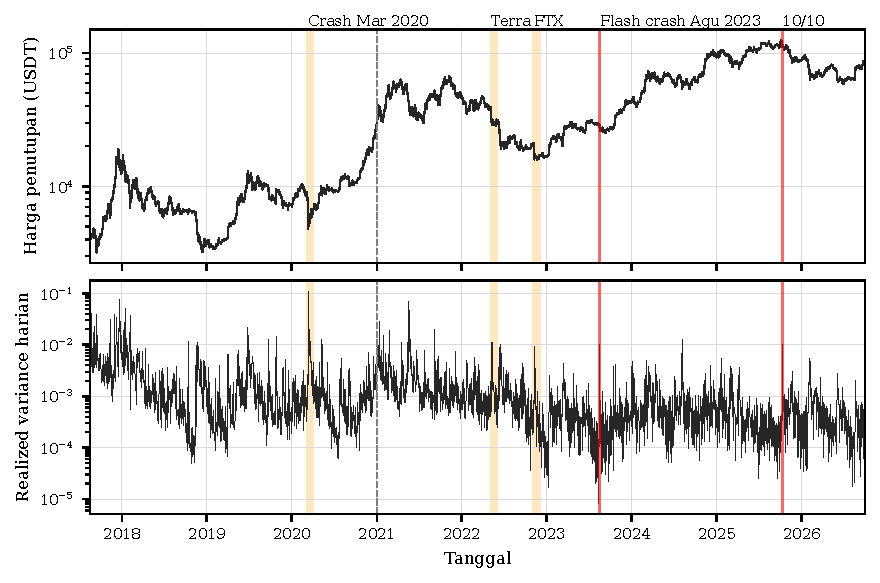
\includegraphics[width=\textwidth]{assets/gambar/gambar-3-2-harga-rv.pdf}
  \caption{Harga Penutupan dan \textit{Realized Variance} Harian BTC/USDT
    Spot, 17 Agustus 2017--30 September 2026}
  \label{fig:data}
\end{figure}

{\small Keterangan: garis putus-putus menandai batas era \textit{transition}
dan \textit{institutional} (1 Januari 2021) mengikuti Do \cite{do2026}; arsir
menandai \textit{crash} Maret 2020, Terra (Mei 2022), dan FTX (November 2022);
garis merah menandai \textit{flash crash} 17 Agustus 2023 dan 10 Oktober 2025
(``10/10''). Sumbu vertikal berskala logaritmik. Sumber: data Binance,
diolah.\par}

\subsection{Audit dan Pra-pemrosesan Data}
\label{subsec:audit}
Tahapan audit adalah sebagai berikut.
\begin{enumerate}
  \item \textbf{Standarisasi \textit{timestamp}.} Arsip Binance sejak
        1 Januari 2025 mencatat waktu dalam mikrodetik, sedangkan arsip
        sebelumnya dalam milidetik; seluruh \textit{timestamp} diseragamkan ke
        milidetik UTC, lalu duplikat dibuang dan data diurutkan.
  \item \textbf{Kelengkapan hari.} Hari dengan jumlah bar kurang dari 95\%
        (kurang dari 274 dari 288 bar) ditandai tidak lengkap. Pasangan
        observasi (fitur hari $t$, target hari $t+1$) dibuang bila hari $t$
        \textbf{atau} hari $t+1$ tidak lengkap atau memiliki RV nol. Sebanyak
        27 hari ditandai tidak lengkap. Sebagai uji sensitivitas, hari-hari
        tersebut dipertahankan.
  \item \textbf{Hari ekstrem dipertahankan} dan tidak dipangkas, karena
        lonjakan volatilitas justru bagian dari fenomena yang diteliti.
  \item \textbf{Volume nol.} Bar dengan volume dolar nol dikecualikan dari
        perhitungan Amihud (Persamaan~\eqref{eq:amihud}).
\end{enumerate}

\subsection{Target dan Fitur}
Target peramalan adalah $RV_{t+1}$ (Persamaan~\eqref{eq:rv}); model dilatih
pada $\ln RV_{t+1}$ lalu ramalannya dikembalikan ke skala level
(Subbab~\ref{subsec:teknis}). Seluruh fitur hari $t$ hanya memakai data hingga
akhir hari $t$. Tiga puluh hari pertama digunakan sebagai periode pemanasan
untuk rata-rata bulanan. Fitur dan model yang memakainya ditunjukkan pada
Tabel~\ref{tab:fitur}.

% CEK: $C_t$ pada baris return harian = harga penutupan bar terakhir hari $t$;
% sudah ditambahkan ke frontmatter/daftar-notasi.tex.
\begin{table}[htbp]
  \caption{Fitur dan Model Pemakainya}
  \label{tab:fitur}
  \centering
  \begingroup
  \setstretch{1}\small
  \begin{tabular}{|p{0.27\textwidth}|p{0.34\textwidth}|p{0.21\textwidth}|}
    \hline
    \textbf{Fitur} & \textbf{Definisi} & \textbf{Dipakai oleh} \\
    \hline
    $\ln RV_t$, $\ln RV^{(w)}_t$, $\ln RV^{(m)}_t$ &
    Persamaan~\eqref{eq:rata-rv}, rata-rata 1, 7, 30 hari & semua model \\
    \hline
    Proporsi semivarians negatif & $RS^-_t / RV_t$,
    Persamaan~\eqref{eq:semivarians} & HAR-X, LGBM-X \\
    \hline
    \textit{Return} harian & $\ln(C_t / C_{t-1})$ & HAR-X, LGBM-X \\
    \hline
    Log volume dolar & $\ln \sum_i QV_{t,i}$ & HAR-X, LGBM-X \\
    \hline
    Perubahan log volume dolar & selisih log volume dolar hari $t$ dan $t-1$ &
    HAR-X, LGBM-X \\
    \hline
    Log \textit{range} Parkinson & $\ln \sigma^2_{P,t}$,
    Persamaan~\eqref{eq:parkinson} & HAR-X, LGBM-X \\
    \hline
    Log Amihud & $\ln \text{Amihud}_t$, Persamaan~\eqref{eq:amihud} &
    LGBM-X \\
    \hline
  \end{tabular}
  \endgroup
\end{table}

Kolinearitas diperiksa dengan \textit{variance inflation factor} (VIF) pada
\textit{window} awal, sebelum fitur dikunci. Log Amihud (VIF 19,6) dan log
volume dolar (VIF 18,2) menunjukkan kolinearitas tinggi; secara konstruksi log
Amihud mendekati setengah $\ln RV$ dikurangi log volume dolar. Sesuai aturan
yang ditetapkan sebelumnya, log Amihud dibuang dari HAR-X saja, sehingga VIF
maksimum fitur X pada HAR-X menjadi 6,9. LGBM-X tetap memakai kesembilan fitur
karena model pohon tidak terpengaruh kolinearitas dalam estimasi.

\subsection{Model}
Model yang digunakan mengikuti desain $2 \times 2$ pada
Tabel~\ref{tab:desain}, ditambah model \textit{naive persistence}
$\widehat{RV}_{t+1} = RV_t$ sebagai pemeriksaan kewajaran.
\begin{itemize}
  \item \textbf{HAR-RV dan HAR-X} diestimasi dengan \textit{ordinary least
        squares} (OLS) pada $\ln RV_{t+1}$ (Persamaan~\eqref{eq:har}); HAR-X
        menambahkan fitur X sebagai regresor.
  \item \textbf{LGBM-HAR dan LGBM-X} menggunakan LightGBM \cite{ke2017} dengan
        \textit{objective} regresi kuadrat, \textit{bagging} 80\% data per
        pohon, dan \textit{hyperparameter} hasil \textit{tuning}
        (Subbab~\ref{subsec:tuning}).
  \item \textbf{Random Forest} dengan masukan yang sama dengan LGBM-X
        (300 pohon, minimum 20 observasi per daun, 33\% fitur per pemisahan)
        digunakan hanya sebagai uji sensitivitas jenis model pohon.
\end{itemize}

\subsection{Aturan Teknis Peramalan}
\label{subsec:teknis}
Aturan berikut berlaku sama untuk semua model.
\begin{enumerate}
  \item \textbf{Koreksi bias transformasi log.} Karena ramalan optimal di
        bawah QLIKE dan MSE adalah nilai harapan kondisional
        \cite{patton2011}, $\exp(\hat y)$ tanpa koreksi akan sistematis
        terlalu rendah. Ramalan dikoreksi menjadi
        $\exp(\hat y_{t+1} + \hat\sigma^2/2)$. Nilai $\hat\sigma^2$ adalah
        varians residual model yang dilatih pada 80\% awal \textit{window}
        latih, dihitung pada 20\% akhir \textit{window}; setelah itu model
        dilatih ulang pada seluruh \textit{window}. Residual
        \textit{in-sample} tidak dipakai karena LightGBM cenderung
        \textit{overfit}.
  \item \textbf{Batas bawah ramalan.} Ramalan dibatasi minimal sebesar
        persentil ke-1 target $RV$ pada \textit{window} latih,
        $\underline{F}$, karena QLIKE menghukum ramalan yang terlalu rendah
        jauh lebih berat \cite{patton2011}.
\end{enumerate}

Ramalan akhir adalah
\begin{equation}
  F_{t+1} = \max\!\left\{
    \exp\!\left(\hat y_{t+1} + \tfrac{1}{2}\hat\sigma^2\right),\;
    \underline{F} \right\}.
  \label{eq:ramalan}
\end{equation}
Sebagai uji sensitivitas, koreksi bias ditiadakan.

\subsection{\textit{Tuning Hyperparameter}}
\label{subsec:tuning}
\textit{Hyperparameter} LightGBM dituning \textbf{sekali} pada \textit{window}
awal (Agustus 2017 -- Agustus 2018) dengan validasi \textit{forward-chaining}
lima lipatan \cite{cerqueira2020}, lalu dikunci untuk seluruh periode
pengujian. Metrik pemilihan adalah rata-rata QLIKE ramalan $\exp(\hat y)$
antarlipatan. Bila kombinasi terbaik berada di tepi ruang pencarian untuk
\texttt{min\_child\_samples} atau \texttt{n\_estimators}, ruang pencarian
diperluas satu langkah ke arah tepi tersebut, maksimal dua kali, dengan batas
bawah \texttt{min\_child\_samples} sebesar 5 untuk menjaga regularisasi. Ruang
pencarian dan nilai terkunci ditunjukkan pada Tabel~\ref{tab:tuning}.

\begin{table}[htbp]
  \caption{Ruang Pencarian dan \textit{Hyperparameter} Terkunci}
  \label{tab:tuning}
  \centering
  \begingroup
  \setstretch{1}\small
  \begin{tabular}{|l|l|c|c|}
    \hline
    \textbf{Parameter} & \textbf{Ruang pencarian awal} & \textbf{LGBM-HAR} &
    \textbf{LGBM-X} \\
    \hline
    \texttt{num\_leaves} & 3, 7, 15 & 3 & 3 \\
    \hline
    \texttt{min\_child\_samples} & 10, 20, 40, 80 & 10 & 5 \\
    \hline
    \texttt{n\_estimators} & 50, 100, 300, 600 & 300 & 300 \\
    \hline
    \texttt{learning\_rate} & 0,03 & 0,03 & 0,03 \\
    \hline
    \texttt{reg\_lambda} & 1, 10 & 1 & 1 \\
    \hline
  \end{tabular}
  \endgroup
\end{table}

Nilai \texttt{min\_child\_samples} = 5 pada LGBM-X merupakan batas bawah ruang
pencarian yang ditetapkan sebelumnya, sehingga dicatat sebagai keputusan
desain untuk menjaga regularisasi.

\subsection{Skema Pembaruan Model (\textit{Walk-Forward})}
Peramalan dilakukan secara \textit{walk-forward} bulanan: pada awal setiap
bulan uji, model dilatih ulang (kecuali S0) menggunakan data dengan tanggal
target sebelum bulan tersebut, lalu meramalkan setiap hari dalam bulan itu.
Ketiga strategi utama mengikuti Tabel~\ref{tab:strategi} dan
Gambar~\ref{fig:strategi}. Model HAR-RV memakai strategi dan \textit{window}
yang sama dengan model ML pada setiap sel perbandingan \cite{chassot2026}.
Awal periode \textit{out-of-sample} setiap skema ditunjukkan pada
Tabel~\ref{tab:oos}; perbandingan antarskema selalu dilakukan pada periode
bersama.

\begin{table}[htbp]
  \caption{Skema Pembaruan dan Awal Periode \textit{Out-of-Sample}}
  \label{tab:oos}
  \centering
  \begingroup
  \setstretch{1}\small
  \begin{tabular}{|l|p{0.34\textwidth}|l|p{0.22\textwidth}|}
    \hline
    \textbf{Skema} & \textbf{Data latih} & \textbf{Awal OOS} &
    \textbf{Peran} \\
    \hline
    S0 & \textit{Window} awal, tidak dilatih ulang & 1 Sep 2018 &
    pembanding manfaat adaptasi \\
    \hline
    S1 & Seluruh data tersedia (\textit{expanding}) & 1 Sep 2018 &
    utama (RQ3) \\
    \hline
    S2-365 & 365 hari terakhir & 1 Sep 2018 & utama (RQ1, RQ2, RQ3) \\
    \hline
    S2-730 & 730 hari terakhir & 1 Sep 2019 & eksploratori \\
    \hline
    S2-180 & 180 hari terakhir & 1 Sep 2018 & eksploratori \\
    \hline
    S2-1095 & 1.095 hari terakhir & 1 Sep 2020 & eksploratori \\
    \hline
    Tertunda-365 & hari ke-730 s.d. ke-365 sebelum bulan uji & 1 Sep 2019 &
    eksploratori (umur data) \\
    \hline
  \end{tabular}
  \endgroup
\end{table}

Pembagian era mengikuti Do \cite{do2026}, dengan batas 1 Januari 2021 antara
era \textit{transition} dan \textit{institutional}; data tahun 2026
diperlakukan sebagai kelanjutan era \textit{institutional} dan diuji
sensitivitasnya. Batas era hanya digunakan dalam analisis, tidak sebagai fitur
model.

\subsection{Kontrol Kebocoran Data}
Langkah pencegahan kebocoran informasi masa depan:
\begin{enumerate}
  \item fitur hari $t$ hanya memakai data hingga akhir hari $t$, sedangkan
        target adalah hari $t+1$;
  \item \textit{tuning} hanya dilakukan pada \textit{window} awal dengan
        \textit{forward-chaining}, bukan validasi silang acak
        \cite{cerqueira2020};
  \item $\hat\sigma^2$ dan batas bawah $\underline{F}$ dihitung hanya dari
        \textit{window} latih;
  \item batas era tidak digunakan sebagai fitur;
  \item tidak ada ambang atau label yang dibentuk dengan melihat data
        \textit{out-of-sample}.
\end{enumerate}

\section{Perhitungan Manual}
Subbab ini memberikan contoh perhitungan satu kali peramalan untuk model
HAR-RV dan LGBM-HAR. Agar tidak memuat hasil pengujian, contoh diambil dari
\textit{window} awal: hari $t^* = $ 30 Agustus 2018 digunakan untuk meramalkan
$RV$ tanggal 31 Agustus 2018, dengan 339 observasi latih (tanggal target
16 September 2017 s.d. 30 Agustus 2018). Seluruh angka ditulis dengan enam
digit bermakna dan telah dicocokkan dengan keluaran implementasi.

\subsection{\textit{Realized Variance} dan Komponen HAR}
\textit{Return} bar pertama hari $t^*$ dihitung terhadap harga penutupan bar
terakhir 29 Agustus 2018, yaitu 7.031,22. Lima bar pertama ditunjukkan pada
Tabel~\ref{tab:manual-rv}.

\begin{table}[htbp]
  \caption{Lima Bar Pertama Hari $t^*$ dan Komponennya}
  \label{tab:manual-rv}
  \centering
  \begingroup
  \setstretch{1}\small
  \begin{tabular}{|l|r|r|r|c|}
    \hline
    \textbf{Waktu (UTC)} & \textbf{Penutupan} & \textbf{$r_{t,i}$} &
    \textbf{$r_{t,i}^2$} & \textbf{$r_{t,i} < 0$} \\
    \hline
    00:00 & 7.038,22 & $9{,}95065 \times 10^{-4}$ &
      $9{,}90153 \times 10^{-7}$ & tidak \\
    \hline
    00:05 & 7.036,24 & $-2{,}81361 \times 10^{-4}$ &
      $7{,}91638 \times 10^{-8}$ & ya \\
    \hline
    00:10 & 7.031,41 & $-6{,}86682 \times 10^{-4}$ &
      $4{,}71532 \times 10^{-7}$ & ya \\
    \hline
    00:15 & 7.039,17 & $1{,}10301 \times 10^{-3}$ &
      $1{,}21663 \times 10^{-6}$ & tidak \\
    \hline
    00:20 & 7.039,01 & $-2{,}27302 \times 10^{-5}$ &
      $5{,}16662 \times 10^{-10}$ & ya \\
    \hline
  \end{tabular}
  \endgroup
\end{table}

Penjumlahan kuadrat \textit{return} atas 288 bar (Persamaan~\eqref{eq:rv})
menghasilkan $RV_{t^*} = 5{,}37199 \times 10^{-4}$. Sebanyak 154 bar memiliki
\textit{return} negatif, sehingga $RS^-_{t^*} = 2{,}67476 \times 10^{-4}$
(Persamaan~\eqref{eq:semivarians}) dan proporsinya
$RS^-_{t^*}/RV_{t^*} = 0{,}497908$.

Komponen HAR dihitung dari rata-rata RV harian, mingguan, dan bulanan
(Persamaan~\eqref{eq:rata-rv}) seperti pada Tabel~\ref{tab:manual-har}.

\begin{table}[htbp]
  \caption{Komponen HAR pada Hari $t^*$}
  \label{tab:manual-har}
  \centering
  \begingroup
  \setstretch{1}\small
  \begin{tabular}{|l|l|}
    \hline
    \textbf{Komponen} & \textbf{Nilai} \\
    \hline
    RV 24 Agustus 2018 & $6{,}28396 \times 10^{-4}$ \\
    \hline
    RV 25 Agustus 2018 & $3{,}50138 \times 10^{-4}$ \\
    \hline
    RV 26 Agustus 2018 & $4{,}82313 \times 10^{-4}$ \\
    \hline
    RV 27 Agustus 2018 & $4{,}99351 \times 10^{-4}$ \\
    \hline
    RV 28 Agustus 2018 & $4{,}54143 \times 10^{-4}$ \\
    \hline
    RV 29 Agustus 2018 & $4{,}40669 \times 10^{-4}$ \\
    \hline
    RV 30 Agustus 2018 ($=RV_{t^*}$) & $5{,}37199 \times 10^{-4}$ \\
    \hline
    Rata-rata mingguan $RV^{(w)}_{t^*}$ & $4{,}84601 \times 10^{-4}$ \\
    \hline
    Bulanan (30 nilai, 1--30 Agustus 2018): minimum &
      $3{,}50138 \times 10^{-4}$ \\
    \hline
    \phantom{Bulanan (30 nilai, 1--30 Agustus 2018): }maksimum &
      $3{,}80630 \times 10^{-3}$ \\
    \hline
    Rata-rata bulanan $RV^{(m)}_{t^*}$ & $1{,}27306 \times 10^{-3}$ \\
    \hline
    $\ln RV_{t^*}$ & $-7{,}52914$ \\
    \hline
    $\ln RV^{(w)}_{t^*}$ & $-7{,}63218$ \\
    \hline
    $\ln RV^{(m)}_{t^*}$ & $-6{,}66633$ \\
    \hline
  \end{tabular}
  \endgroup
\end{table}

\subsection{Fitur X}
Keenam fitur X pada hari $t^*$ ditunjukkan pada Tabel~\ref{tab:manual-x}.
Model HAR-X tidak memakai log Amihud, sesuai hasil pemeriksaan VIF pada
Subbab~\ref{subsec:audit}; fitur tersebut hanya dipakai LGBM-X.

\begin{table}[htbp]
  \caption{Fitur X pada Hari $t^*$}
  \label{tab:manual-x}
  \centering
  \begingroup
  \setstretch{1}\small
  \begin{tabular}{|p{0.26\textwidth}|p{0.34\textwidth}|p{0.26\textwidth}|}
    \hline
    \textbf{Fitur} & \textbf{Masukan mentah} & \textbf{Hasil} \\
    \hline
    \textit{Return} harian & penutupan $t^*$ = 6.984,84; penutupan $t^*-1$ =
      7.031,22 & $-0{,}00661815$ \\
    \hline
    Log volume dolar & volume dolar $t^*$ = $3{,}09357 \times 10^{8}$ &
      19,5500 \\
    \hline
    Perubahan log volume dolar & volume dolar $t^*-1$ =
      $3{,}04565 \times 10^{8}$ & $19{,}5500 - 19{,}5344 = 0{,}0156107$ \\
    \hline
    Log \textit{range} Parkinson & $P^H_{t^*}$ = 7.063,63;
      $P^L_{t^*}$ = 6.784,81 & $-7{,}44394$ \\
    \hline
    Log Amihud & $10^6 \times$ rata-rata $|r_{t,i}|/QV_{t,i}$ =
      $0{,}00116494$ & $-6{,}75508$ \\
    \hline
    Proporsi semivarians negatif & lihat Subbab 3.3.1 & 0,497908 \\
    \hline
  \end{tabular}
  \endgroup
\end{table}

\subsection{Peramalan HAR-RV dan LGBM-HAR}
Koefisien HAR-RV hasil OLS pada \textit{window} latih adalah
$\beta_0 = -0{,}569890$, $\beta_d = 0{,}478542$, $\beta_w = 0{,}0689003$, dan
$\beta_m = 0{,}384379$. Dengan Persamaan~\eqref{eq:har},
\begin{align}
  \hat y_{t^*+1} &= (-0{,}569890)
    + (0{,}478542)(-7{,}52914)
    + (0{,}0689003)(-7{,}63218) \nonumber \\
  &\quad + (0{,}384379)(-6{,}66633) \nonumber \\
  &= (-0{,}569890) + (-3{,}60301) + (-0{,}525859) + (-2{,}56240) \nonumber \\
  &= -7{,}26116 .
  \label{eq:manual-har}
\end{align}
Varians residual $\hat\sigma^2 = 0{,}497938$ diperoleh dari model yang dilatih
pada 271 observasi awal dan dievaluasi pada 68 observasi akhir. Dengan
Persamaan~\eqref{eq:ramalan},
$\exp(-7{,}26116 + 0{,}248969) = 9{,}00836 \times 10^{-4}$, yang berada di
atas batas bawah $\underline{F} = 2{,}90955 \times 10^{-4}$, sehingga
$F_{\text{HAR}} = 9{,}00836 \times 10^{-4}$.

Pada LGBM-HAR, nilai awal berupa rata-rata $\ln RV_{t+1}$ data latih,
$-6{,}03756$, dilebur ke nilai daun pohon pertama, sehingga $\hat y$ merupakan
jumlah nilai daun dari 300 pohon (Persamaan~\eqref{eq:gbdt}). Struktur dua
pohon pertama beserta lintasan hari $t^*$ ditunjukkan pada
Gambar~\ref{fig:manual-pohon}.

% CEK: jumlah n per daun pohon ke-1 (256) tidak konsisten dengan bagging 80%
% dari 339 obs (~271); sedang dicek di chat script. Karena itu n tidak
% ditampilkan.
\begin{figure}[htbp]
  \centering
  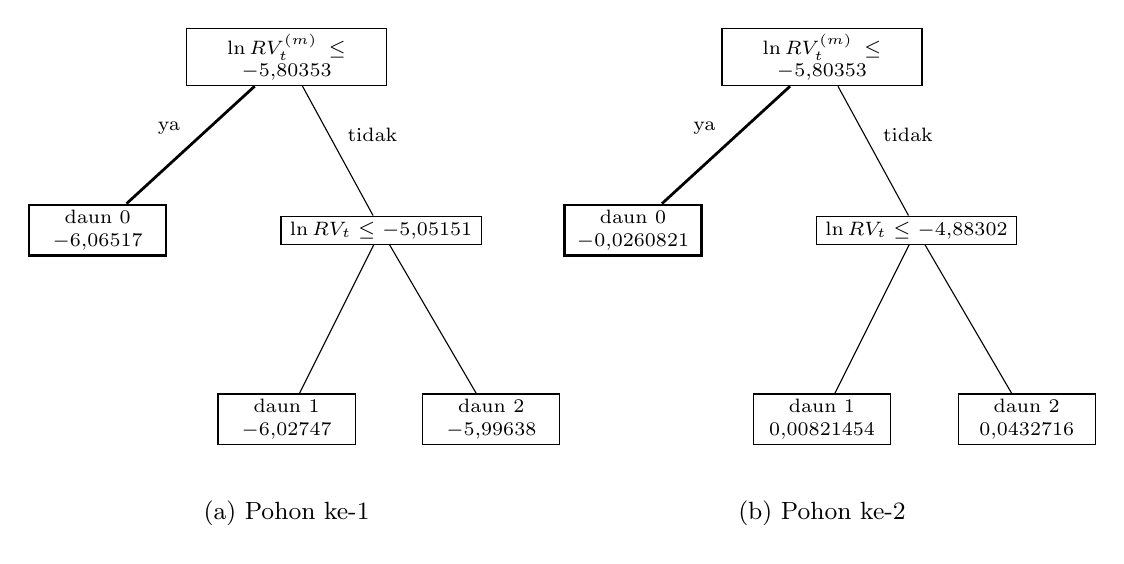
\begin{tikzpicture}[x=1mm,y=-1mm,
      simpul/.style={draw,align=center,inner sep=2pt,font=\scriptsize,
        text width=24mm},
      daun/.style={draw,align=center,inner sep=2pt,font=\scriptsize,
        text width=16mm},
      tebal/.style={line width=1pt}]

    % Panel kiri: pohon ke-1
    \begin{scope}
      \node[simpul] (a) at (30,0) {$\ln RV^{(m)}_t \le -5{,}80353$};
      \node[daun,tebal] (a0) at (6,22) {daun 0\\$-6{,}06517$};
      \node[simpul] (a1) at (42,22) {$\ln RV_t \le -5{,}05151$};
      \node[daun] (a11) at (30,46) {daun 1\\$-6{,}02747$};
      \node[daun] (a12) at (56,46) {daun 2\\$-5{,}99638$};
      \draw[tebal] (a) -- node[above left,font=\scriptsize] {ya} (a0);
      \draw (a) -- node[above right,font=\scriptsize] {tidak} (a1);
      \draw (a1) -- (a11);
      \draw (a1) -- (a12);
      \node[font=\small] at (30,58) {(a) Pohon ke-1};
    \end{scope}

    % Panel kanan: pohon ke-2
    \begin{scope}[xshift=68mm]
      \node[simpul] (b) at (30,0) {$\ln RV^{(m)}_t \le -5{,}80353$};
      \node[daun,tebal] (b0) at (6,22) {daun 0\\$-0{,}0260821$};
      \node[simpul] (b1) at (42,22) {$\ln RV_t \le -4{,}88302$};
      \node[daun] (b11) at (30,46) {daun 1\\$0{,}00821454$};
      \node[daun] (b12) at (56,46) {daun 2\\$0{,}0432716$};
      \draw[tebal] (b) -- node[above left,font=\scriptsize] {ya} (b0);
      \draw (b) -- node[above right,font=\scriptsize] {tidak} (b1);
      \draw (b1) -- (b11);
      \draw (b1) -- (b12);
      \node[font=\small] at (30,58) {(b) Pohon ke-2};
    \end{scope}
  \end{tikzpicture}
  \caption{Struktur Pohon ke-1 dan ke-2 LGBM-HAR pada Contoh Perhitungan}
  \label{fig:manual-pohon}
  \sumber{Garis tebal menandai lintasan hari $t^*$, dengan
    $\ln RV^{(m)}_{t^*} = -6{,}66633$}
\end{figure}

Hari $t^*$ memiliki $\ln RV^{(m)}_{t^*} = -6{,}66633$, yang memenuhi syarat
pemisahan pertama pada kedua pohon, sehingga keduanya berakhir di daun 0.
Kontribusi pohon ke-1 adalah $-6{,}06517$, yaitu gabungan nilai awal
$-6{,}03756$ dan nilai daun $-0{,}0276166$; kontribusi pohon ke-2 adalah
$-0{,}0260821$; dan jumlah kontribusi pohon ke-3 hingga ke-300 adalah
$-1{,}22919$. Total ketiganya menghasilkan $\hat y_{t^*+1} = -7{,}32044$.
Dengan $\hat\sigma^2 = 0{,}511547$, diperoleh
$\exp(-7{,}32044 + 0{,}255773) = 8{,}54778 \times 10^{-4}$, yang juga di atas
batas bawah, sehingga $F_{\text{LGBM}} = 8{,}54778 \times 10^{-4}$.

\subsection{Evaluasi Satu Hari}
\textit{Realized variance} aktual tanggal 31 Agustus 2018 adalah
$4{,}14190 \times 10^{-4}$. Nilai \textit{loss} kedua model dihitung dengan
Persamaan~\eqref{eq:loss} dan ditunjukkan pada Tabel~\ref{tab:manual-loss}.

\begin{table}[htbp]
  \caption{Evaluasi Ramalan 31 Agustus 2018}
  \label{tab:manual-loss}
  \centering
  \begingroup
  \setstretch{1}\small
  \begin{tabular}{|l|l|l|l|l|}
    \hline
    \textbf{Model} & \textbf{$F_{t+1}$} & \textbf{$RV_{t+1}/F_{t+1}$} &
    \textbf{QLIKE} & \textbf{MSE} \\
    \hline
    HAR-RV & $9{,}00836 \times 10^{-4}$ & 0,459784 & 0,236783 &
      $2{,}36825 \times 10^{-7}$ \\
    \hline
    LGBM-HAR & $8{,}54778 \times 10^{-4}$ & 0,484558 & 0,209076 &
      $1{,}94118 \times 10^{-7}$ \\
    \hline
  \end{tabular}
  \endgroup
\end{table}

Selisih \textit{loss} pada hari tersebut (Persamaan~\eqref{eq:delta-loss})
adalah $\Delta L = 0{,}209076 - 0{,}236783 = -0{,}0277067$. Nilai negatif
menunjukkan LGBM-HAR lebih akurat \textbf{pada hari contoh ini saja}; satu
hari tidak dapat dijadikan dasar kesimpulan, sehingga pengujian dilakukan atas
seluruh periode \textit{out-of-sample} sebagaimana diuraikan pada Subbab 3.4.

\section{Evaluasi dan Pengujian Hipotesis}

\subsection{Fungsi \textit{Loss} dan Selisih \textit{Loss}}
Setiap ramalan dievaluasi dengan QLIKE sebagai \textit{loss} utama dan MSE
pada skala level sebagai pelengkap (Persamaan~\eqref{eq:loss}). Objek analisis
adalah selisih \textit{loss} harian $\Delta L_t$
(Persamaan~\eqref{eq:delta-loss}). Pasangan konfirmatori adalah LGBM-X
terhadap HAR-RV pada skema S2-365; pasangan lain, yaitu LGBM-HAR--HAR,
HAR-X--HAR, LGBM-X--LGBM-HAR, dan LGBM-X--HAR-X, digunakan untuk dekomposisi
secara eksploratori.

\subsection{Uji Konfirmatori}
Uji konfirmatori setiap hipotesis mengikuti Tabel~\ref{tab:ringkasan}.
Rincian pelaksanaannya adalah sebagai berikut.
\begin{enumerate}
  \item \textbf{RQ1.} UDmax (Persamaan~\eqref{eq:udmax}) pada rata-rata
        $\Delta L_t$ dengan \textit{trimming} $\varepsilon = 0{,}15$ dan
        maksimum lima perubahan, statistik Wald memakai kovarians HAC
        \cite{bai1998,bai2003,martins2016}. Bila UDmax tidak menolak $H_0$,
        dilanjutkan dengan uji tipe Diebold--Mariano
        (Persamaan~\eqref{eq:dm}) pada seluruh sampel.
  \item \textbf{RQ2.} H2a diuji dengan regresi rata-rata $\Delta L$ bulanan
        pada empat karakteristik pasar (Subbab~\ref{subsec:rq2var}), dengan
        uji-F bersama berbasis kovarians HAC. H2b diuji dengan regresi
        $\Delta L_t = \alpha + \delta\,\text{Era}_t + e_t$ untuk dua
        pasangan kontribusi fitur X (HAR-X--HAR dan LGBM-X--LGBM-HAR), uji-t
        HAC pada $\delta$, dengan koreksi Holm atas dua uji tersebut
        \cite{holm1979}.
  \item \textbf{RQ3.} Uji-t HAC dua sisi pada rata-rata $D_t$ (Subbab 2.4) di
        era \textit{institutional}, pada periode bersama S2-365 dan S1. H3
        didukung bila rata-rata $D_t$ negatif dan signifikan; rata-rata
        positif yang signifikan dibaca sebagai dukungan bagi hipotesis
        tandingan.
\end{enumerate}

Semua uji menggunakan taraf signifikansi 5\% dan kovarians HAC Newey--West
dengan kernel Bartlett dan \textit{bandwidth} otomatis Andrews
\cite{newey1987,andrews1991}.

Nilai kritis UDmax, uji perubahan berurutan, dan \textit{Fluctuation test}
diperoleh dengan simulasi Monte Carlo, bukan dikutip dari tabel: 3.000
replikasi deret normal baku sepanjang 1.000 observasi untuk UDmax, dan 5.000
replikasi gerak Brown diskret untuk \textit{Fluctuation test}.
\textit{p-value} dihitung sebagai $(R^{+}+1)/(R+1)$, dengan $R^{+}$ jumlah
statistik simulasi yang tidak lebih kecil dari statistik amatan dan $R$ jumlah
replikasi. Nilai kritis simulasi dibandingkan
dengan tabel Bai--Perron sebagai pemeriksaan \cite{bai1998}.

% CEK: tabel asli Bai--Perron (1998) untuk q = 1, epsilon = 0,15 belum
% dicocokkan langsung.

\subsection{Variabel Karakteristik Pasar (RQ2)}
\label{subsec:rq2var}
Untuk setiap bulan uji dihitung empat variabel seperti pada
Tabel~\ref{tab:rq2var}.

\begin{table}[htbp]
  \caption{Variabel Karakteristik Pasar Bulanan}
  \label{tab:rq2var}
  \centering
  \begingroup
  \setstretch{1}\small
  \begin{tabular}{|p{0.3\textwidth}|p{0.55\textwidth}|}
    \hline
    \textbf{Variabel} & \textbf{Definisi} \\
    \hline
    Level volatilitas & rata-rata $\ln RV_t$ dalam bulan \\
    \hline
    Volatilitas dari volatilitas & deviasi standar $\ln RV_t$ dalam bulan \\
    \hline
    Likuiditas & rata-rata \textit{spread} Abdi--Ranaldo harian
      \cite{abdi2017} \\
    \hline
    Pergeseran distribusi fitur & rata-rata $D^{\text{KS}}$
      (Persamaan~\eqref{eq:ks}) antara \textit{window} latih S2-365 dan bulan
      uji atas sembilan fitur LGBM-X \\
    \hline
  \end{tabular}
  \endgroup
\end{table}

\textit{Spread} Abdi--Ranaldo harian dihitung sebagai
\begin{equation}
  s_t = \sqrt{\max\{4\,(c_t - \bar{p}_t)(c_t - \bar{p}_{t+1}),\, 0\}},
  \label{eq:abdi}
\end{equation}
dengan $\bar{p}_t = (\ln P^H_t + \ln P^L_t)/2$ dan $c_t$ logaritma harga
penutupan hari $t$. Nilai negatif di bawah akar dijadikan nol sebelum
dirata-rata. Sebagai uji sensitivitas, estimator Corwin--Schultz
\cite{corwin2012} digunakan sebagai pengganti. Sebagai pelengkap deskriptif,
dihitung pula \textit{population stability index} (PSI) antara \textit{window}
latih dan bulan uji.

Regresi H2a dirumuskan sebagai
\begin{equation}
  \overline{\Delta L}_\tau = \alpha + \sum_{k=1}^{4} \gamma_k\, z_{k,\tau}
    + \delta\, \text{Era}_\tau + u_\tau,
  \label{eq:rq2}
\end{equation}
dengan $\overline{\Delta L}_\tau$ rata-rata $\Delta L_t$ bulan $\tau$,
$z_{k,\tau}$ keempat variabel pada Tabel~\ref{tab:rq2var}, dan
$\text{Era}_\tau$ variabel \textit{dummy} era \textit{institutional} yang
selalu disertakan. Untuk menghindari regresi palsu, setiap regresor diuji
dengan ADF \cite{dickey1979} dan KPSS \cite{kwiatkowski1992}; regresor
di-\textit{differencing} bila ADF gagal menolak akar unit ($p > 0{,}05$)
\textbf{dan} KPSS menolak stasioneritas ($p < 0{,}05$). Hipotesis yang diuji
adalah $\gamma_1 = \gamma_2 = \gamma_3 = \gamma_4 = 0$. Interpretasi bersifat
asosiatif, bukan kausal.

\subsection{Analisis Eksploratori}
Analisis berikut bersifat eksploratori dan \textit{p-value}-nya dikoreksi
dengan prosedur Holm per keluarga rumusan masalah \cite{holm1979}:
\begin{enumerate}
  \item uji perubahan berurutan $\sup F(\ell+1 \mid \ell)$ untuk menentukan
        jumlah dan tanggal perubahan \cite{bai2003};
  \item \textit{Fluctuation test} dengan $\mu = 0{,}3$ dan $0{,}2$ sebagai
        grafik deskriptif \cite{giacomini2010};
  \item pasangan dekomposisi, skema S0 dan S2 lain, serta \textit{loss} MSE;
  \item kurva panjang \textit{window} (S2-180 s.d. S1) dan perbandingan efek
        jumlah data (S2-730 terhadap S2-365) dengan efek umur data
        (Tertunda-365 terhadap S2-365);
  \item analisis daya UDmax dengan \textit{bootstrap} blok 30 hari.
\end{enumerate}

\subsection{Uji Sensitivitas}
Kesimpulan konfirmatori diperiksa terhadap variasi pada
Tabel~\ref{tab:sensitivitas}.

% CEK: sensitivitas RV 5 menit subsampled (butuh data 1 menit) dan retuning
% tahunan ada di rencana v2.5 tetapi belum dijalankan. Tambahkan ke tabel
% hanya jika Ferdi memutuskan akan menjalankannya.
\begin{table}[htbp]
  \caption{Variasi Uji Sensitivitas}
  \label{tab:sensitivitas}
  \centering
  \begingroup
  \setstretch{1}\small
  \begin{tabular}{|p{0.3\textwidth}|p{0.55\textwidth}|}
    \hline
    \textbf{Variasi} & \textbf{Perubahan terhadap desain utama} \\
    \hline
    Tanpa 2026 & data uji dibatasi hingga 31 Desember 2025 \\
    \hline
    Hari tidak lengkap dipertahankan & aturan audit
      Subbab~\ref{subsec:audit} butir 2 tidak diterapkan \\
    \hline
    \textit{Window} awal 24 bulan & \textit{tuning} dan awal OOS memakai
      \textit{window} awal 730 hari \\
    \hline
    Lag 1, 5, 22 & horizon HAR mengikuti hari perdagangan saham \\
    \hline
    Random Forest & LGBM-X diganti Random Forest \\
    \hline
    RV 15 menit & target dan fitur HAR dari \textit{return} 15 menit \\
    \hline
    Tanpa koreksi bias & $\hat\sigma^2 = 0$ pada
      Persamaan~\eqref{eq:ramalan} \\
    \hline
    HAR re-estimasi harian & HAR dilatih ulang setiap hari, bukan bulanan \\
    \hline
    Likuiditas Corwin--Schultz & khusus H2a \\
    \hline
  \end{tabular}
  \endgroup
\end{table}

\section{Jadwal Penelitian}
Jadwal pelaksanaan penelitian ditunjukkan pada Tabel~\ref{tab:jadwal}.

% CEK: kolom bulan dan tanda centang diisi Ferdi sesuai rencana dan kalender
% prodi. Jangan menebak durasi.
\begin{table}[htbp]
  \caption{Jadwal penelitian}
  \label{tab:jadwal}
  \centering
  \begingroup
  \setstretch{1}
  \begin{tabular}{|c|p{0.45\textwidth}|c|c|c|c|}
    \hline
    \textbf{No} & \textbf{Kegiatan} & \textbf{Bln 1} & \textbf{Bln 2} &
    \textbf{Bln 3} & \textbf{Bln 4} \\
    \hline
    1 & Studi literatur dan verifikasi kebaruan & & & & \\
    \hline
    2 & Pengumpulan dan audit data & & & & \\
    \hline
    3 & Uji kelayakan (\textit{pilot}) & & & & \\
    \hline
    4 & Implementasi \textit{pipeline} dan eksperimen & & & & \\
    \hline
    5 & Analisis dan pengujian hipotesis & & & & \\
    \hline
    6 & Penulisan Bab IV dan V & & & & \\
    \hline
    7 & Seminar hasil dan sidang & & & & \\
    \hline
  \end{tabular}
  \endgroup
\end{table}


\daftarpustaka

\input{appendices/lampiran-1}
\end{document}
